%  LaTeX support: latex@mdpi.com
%=================================================================
\documentclass[sensors,article,submit,moreauthors,pdftex]{Definitions/mdpi}

%=================================================================
% MDPI frontmatter
\firstpage{1}
\makeatletter
\setcounter{page}{\@firstpage}
\makeatother
\pubvolume{1}
\issuenum{1}
\articlenumber{0}
\pubyear{2026}
\copyrightyear{2026}
\history{Received: date; Accepted: date; Published: date}

%=================================================================
% Additional packages
\usepackage{booktabs}
\usepackage{multirow}
\usepackage{amsmath}
\usepackage{amssymb}

% Custom commands
\newcommand{\ie}{\textit{i.e.}}
\newcommand{\eg}{\textit{e.g.}}
\newcommand{\etal}{\textit{et al.}}

% ORCID
\newcommand{\orcidauthorA}{0009-0009-0292-9706}

%=================================================================
% Title
\Title{Multi-Scale Sensor-to-G-Code Reconstruction Mismatch for CNC Anomaly Detection}

% Authors
\Author{Stephen S. Eacuello $^{1,}$*\orcidA{}, Romesh S. Prasad $^{1}$ and Manbir S. Sodhi $^{1}$}

\AuthorNames{Stephen S. Eacuello, Romesh S. Prasad and Manbir S. Sodhi}

% Affiliations
\address{%
$^{1}$ \quad Department of Industrial Systems Engineering, University of Rhode Island, Kingston, RI 02881, USA}

% Corresponding author
\corres{Correspondence: seacuello@uri.edu}

% Abstract
\abstract{A CNC program altered by a fraction of a millimeter in one coordinate or by one swapped motion command can produce parts that pass visual inspection but fail under load. Existing sensor-based monitoring cannot detect this because the modified program remains physically valid and sensor signals stay within the normal machining distribution. We train a decoder to reconstruct G-code from sensor signals; disagreement between the claimed program and the reconstruction indicates tampering. At 4~Hz effective sampling, the signals encode program structure and quasi-static process state, not cutting-force spectra. No single detection strategy covers all attack types. Short-context decoding detects command-level tampering, multi-line decoding detects cross-operation swaps, and rank-based scoring, invariant to absolute probability magnitudes, recovers coordinate-perturbation detection where likelihood scoring fails ($p \leq 1.2\times10^{-5}$, DeLong test, Holm-corrected). Sensor-only baselines have no genuine detection signal because the attacks leave the sensors unchanged. The detector runs on six \$33 sensor boards, decoder inference under 6~ms per window ($11{,}000\times$ real-time on a GPU). We report negative results (multi-head disagreement scoring, temperature-scaled calibration, CUSUM temporal detection), a per-token confidence analysis explaining the coordinate-attack detection limit, and an adaptive-adversary evaluation where single-score detection drops to near chance.}

% Keywords
\keyword{CNC machining; anomaly detection; G-code reconstruction; side-channel sensor fusion; autoregressive decoder; manufacturing cybersecurity}

\begin{document}

\section{Introduction}
\label{sec:introduction}

Computer numerical control (CNC) machining underpins precision manufacturing in aerospace, automotive, medical, and defense sectors, where dimensional deviations as small as 0.05~mm can render safety-critical parts non-functional~\cite{nist2023,graves2023cyberphysical}.
As manufacturing systems adopt Industry~4.0 architectures, cloud-based CAM, and remote monitoring, they inherit the cybersecurity vulnerabilities of general-purpose IT while retaining the physical consequences unique to operational technology (OT).
NIST SP 800-82 Rev.~3 identifies CNC controllers as critical OT assets requiring integrity verification~\cite{nist2023}, and the Cybersecurity Manufacturing Innovation Institute (CyManII) has prioritized CNC attack detection as a national research need~\cite{cymanii2022}.

The canonical cyber-physical attack modifies the G-code program (the motion and machine-control commands defining the manufacturing process) either in transit or at rest on the controller's file system~\cite{yampolskiy2018security,belikovetsky2017dr0wned}.
Even simple modifications (replacing a coordinate value, swapping a motion command, altering a feed rate) can produce parts that pass visual inspection but fail under load~\cite{belikovetsky2017dr0wned,zeltmann2016manufacturing}, as documented by the MITRE ATT\&CK for ICS framework under the ``Impair Process Control'' tactic~\cite{mitre2021attack}.

Existing CNC monitoring performs \emph{process classification} rather than \emph{integrity verification}.
Classification approaches assign sensor signals to known toolpath categories but cannot verify that the physically executed process matches the commanded program.
An adversary who modifies G-code to produce a slightly altered but physically valid toolpath (e.g., shifting a coordinate by 0.1~in or substituting one operation for another) generates sensor signals that remain within the distribution of normal machining, evading classification-based detectors entirely.

We propose a \emph{reconstruction-mismatch} approach to CNC anomaly detection.
A model trained to reconstruct G-code token sequences from multi-modal sensor signals learns the conditional distribution $p(\mathbf{y} \mid \mathbf{z})$ mapping sensor-derived latent representations $\mathbf{z}$ to G-code tokens $\mathbf{y}$.
When an attacker modifies the G-code, the sensor signals still reflect the \emph{original} physical process.
The decoder therefore reconstructs the correct tokens with high probability while assigning low probability to the substituted tokens.
The discrepancy between reconstruction and claimed G-code provides the detection signal.

This approach extends reconstruction-based anomaly detection~\cite{an2015variational,chalapathy2019deep} in three domain-specific ways.
First, the reconstruction target is a \emph{structured token sequence} (G-code), enabling language-model scoring methods (NLL, rank-based metrics, perplexity).
Second, multi-modal sensor input (accelerometers, gyroscopes, magnetometers, audio, environmental sensors, and electrical measurements across six sensor boards) constrains the reconstruction space far more than any single modality.
Third, the G-code grammar partitions attacks into \emph{grammar-violating} (trivially detectable by parsing) and \emph{grammar-compliant} (the hard, security-relevant case) categories, focusing evaluation on attacks that require learned representations.

The deployable \emph{unsupervised} detector reaches AUROC 0.803 on command-swap attacks (V7 NLL), 0.859 on small coordinate perturbations (V7 rank scoring), and 0.949 on cross-operation swaps (V8 NLL).
Sensor-only baselines, in contrast, lack a genuine detection signal against these G-code integrity attacks.
A supervised XGBoost classifier raises small-coordinate detection to 0.962 when labeled attacks are available; we report this as an upper bound rather than as the deployable result.
A per-token confidence analysis, an adaptive-adversary evaluation, and a calibration study characterize the limits of the approach.

The contributions of this paper are:

\begin{enumerate}
    \item \textbf{Multi-scale reconstruction-mismatch framework.} We combine a frozen multi-modal encoder (MM-DTAE-LSTM, 110 sensor channels) with two autoregressive decoder scales, short-context (V7) and multi-line (V8), and with rank-based scoring and ensemble methods, to detect grammar-compliant G-code attacks from sensor signals alone.

    \item \textbf{Supervised upper bound.} A supervised XGBoost classifier trained on features combining encoder memory, NLL statistics, and rank scores achieves AUROC 0.962 on small coordinate attacks when labeled attacks are available; we present this as an upper bound, not the deployable system. An unsupervised grid-searched ensemble only matches the best individual scorer per attack type (in-sample AUROC up to 0.859).

    \item \textbf{Baseline inadequacy.} We show that sensor-only baselines have no genuine detection signal for G-code integrity attacks. Because the attack leaves the physical process and every sensor channel unchanged, a \emph{paired} sensor-space comparison is exactly at chance, and the near-chance unpaired baselines we report deviate from 0.50 only through window-selection artifacts, not detection. The detection signal must instead come from comparing sensor observations against the \emph{claimed} program, which is what reconstruction-mismatch does.

    \item \textbf{Characterization of detection limits.} A per-token confidence analysis shows that detectability rises smoothly with the decoder's confidence; confident tokens (54\% of positions) reach per-token AUROC 0.89 while low-confidence tokens are near chance. We evaluate a first-order adaptive adversary that drives single-score detection to near chance (AUROC 0.54). We further document calibration failures (temperature scaling degrades ECE for the multi-line decoder) and identify a position confound affecting coordinate-attack evaluation.
\end{enumerate}

Code and trained models are available at [URL redacted for review].

\section{Related Work}
\label{sec:related_work}

\subsection{CNC Process Monitoring and Attack Detection}
\label{sec:rw_cnc_anomaly}

CNC process monitoring has traditionally focused on tool wear, chatter, and surface quality prediction using vibration, acoustic emission, and cutting force signals~\cite{teti2010advanced,dimla2000sensor}.
Cuka and Kim~\cite{cuka2022fuzzy} demonstrated fuzzy logic-based tool condition monitoring via multi-sensor fusion, and Wang et al.~\cite{wang2023deep} surveyed the shift from hand-crafted statistical features to deep learning representations for process monitoring.

More recently, researchers have addressed \emph{adversarial} threats to CNC systems.
Energy-based methods monitor spindle power to detect unauthorized G-code modifications~\cite{kimmell2025}, achieving strong detection of gross toolpath changes but missing subtle coordinate perturbations that preserve the power envelope.
CNN-based vibration analysis~\cite{coelho2024} detects tool breakage and collisions but requires retraining on labeled anomaly examples for each new attack type.
The broader manufacturing cybersecurity literature has documented the threat landscape: Yampolskiy et al.~\cite{yampolskiy2018security} taxonomized additive manufacturing attacks by surface and impact; Belikovetsky et al.~\cite{belikovetsky2017dr0wned} demonstrated a complete attack chain inducing fatigue failure while maintaining external conformance; Graves et al.~\cite{graves2023cyberphysical} identified G-code integrity verification as an open problem.

The critical gap is the distinction between \emph{fault detection} and \emph{integrity verification}.
Process monitoring detects deviations from expected statistical behavior but does not verify that what was executed matches what was \emph{commanded}.
An adversary producing a slightly different but physically plausible toolpath may evade fault detectors entirely, because the process appears ``normal''---it is simply the wrong program.
Our reconstruction-mismatch approach addresses this gap by learning the inverse mapping from sensor signals to G-code, detecting any discrepancy between commanded and executed programs.

\subsection{Manufacturing Side-Channel Analysis}
\label{sec:rw_sidechannel}

Offensive side-channel research has shown that CNC and additive manufacturing processes leak substantial information through acoustic, electromagnetic, and power channels.
Acoustic emissions can reconstruct 3D printer toolpath geometry with sub-millimeter accuracy~\cite{al2016acoustic}; even a nearby smartphone captures sufficient data to reconstruct printed geometry~\cite{hojjati2016leave}.
Actuator power signatures can detect sabotage in additive manufacturing~\cite{gatlin2019detecting}, and spindle power profiles discriminate gross toolpath changes but not small coordinate perturbations~\cite{moore2017power}.

Our work \emph{inverts} this paradigm: rather than extracting proprietary information from sensor signals (IP theft), we use sensor signals to \emph{verify} G-code integrity (defensive monitoring).
This leverages the same physical coupling between machining parameters and sensor responses, applied for security rather than espionage.
The closest analogue is network intrusion detection via language-model perplexity on protocol sequences~\cite{brown2018recurrent}---we apply the same principle to G-code tokens reconstructed from physical sensor measurements.

\subsection{Sequence-Level Anomaly Detection}
\label{sec:rw_sequence_anomaly}

Reconstruction-error-based anomaly detection is well established~\cite{chalapathy2019deep}: autoencoders threshold reconstruction loss to identify out-of-distribution inputs~\cite{an2015variational}, while LSTMs with dynamic thresholding capture temporal dependencies in spacecraft telemetry~\cite{hundman2018detecting}, and Transformer architectures such as TranAD use self-conditioning and adversarial training for multivariate time-series anomaly detection~\cite{tuli2022tranad}.
In the discrete domain, language models score anomalies via perplexity or NLL, flagging ``surprising'' sequences~\cite{brown2018recurrent}, an approach successfully applied to system log anomaly detection.

Our reconstruction target differs from both continuous time series and free-form text: G-code is a \emph{structured token sequence} with strict grammar.
Each line begins with a command token (G0, G1, etc.) followed by parameter--value pairs, where parameter letters and numeric values occupy distinct fields.
This structure provides an additional grammar-violation detection signal unavailable in other domains, and motivates our multi-head decoder with separate heads for token type, command, parameter, and numeric value.
No prior work has applied autoregressive token-level anomaly scoring to G-code sequences reconstructed from multi-modal sensor inputs; the closest analog uses language models for IT log-file anomaly detection~\cite{brown2018recurrent}, which lacks G-code's mixed vocabulary and grammatical constraints.

\subsection{Calibration and Confidence Estimation}
\label{sec:rw_calibration}

Modern neural networks are often poorly calibrated: softmax probabilities do not reflect true predictive accuracy~\cite{guo2017calibration}.
Temperature scaling---a single learned scalar on a validation set---is widely recommended as a default calibration strategy~\cite{guo2017calibration,platt1999probabilistic,naeini2015obtaining}.
For anomaly detection, calibration matters because thresholds are set from score distributions; miscalibrated scores make operating-point selection unreliable.
OOD detection methods based on softmax thresholding~\cite{hendrycks2017baseline}, Mahalanobis distance~\cite{lee2018simple}, ODIN perturbation~\cite{liang2018enhancing}, and energy scoring~\cite{liu2020energy} all depend on well-calibrated confidence estimates.

As we show in Section~\ref{sec:results_calibration}, temperature scaling produces mixed results on our decoder, cautioning against uncritical application of post-hoc calibration methods.

\section{System Architecture}
\label{sec:architecture}

The detection system has two stages: a multi-modal encoder mapping raw sensor signals to a latent representation, and an autoregressive decoder reconstructing the G-code token sequence from this representation (Fig.~\ref{fig:architecture}).
The encoder is pre-trained and frozen; only the decoder is trained for reconstruction.
At inference, anomalies are detected by comparing the decoder's reconstruction against the claimed G-code and computing an anomaly score from the discrepancy.

\begin{figure}[t]
    \centering
    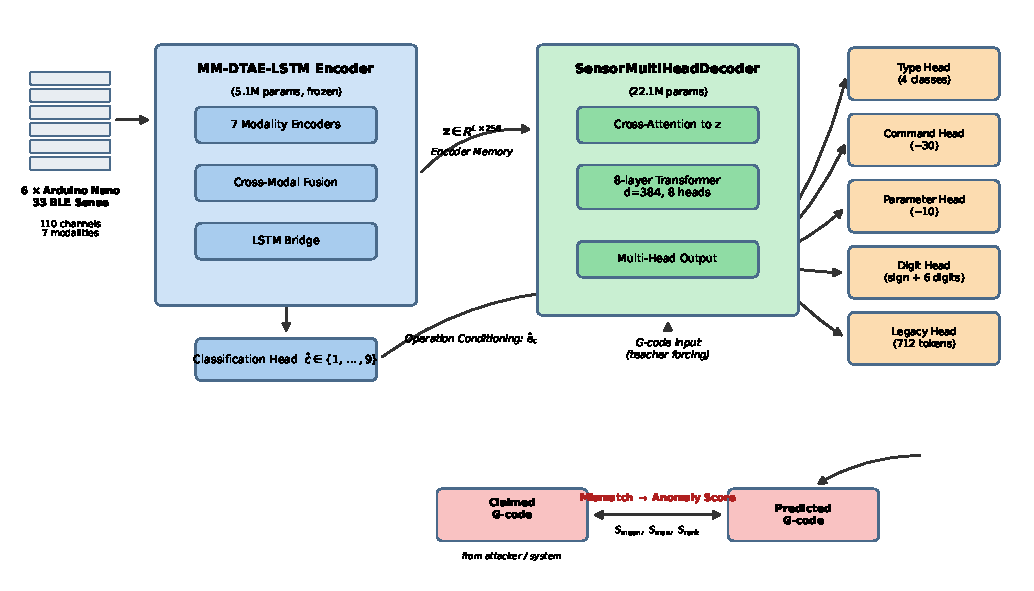
\includegraphics[width=\textwidth]{figures/architecture_overview}
    \caption{System architecture overview. Sensor signals from six Arduino-based boards (110 channels, seven modality groups) are encoded by the frozen MM-DTAE-LSTM encoder into a latent sequence $\mathbf{z}$. The autoregressive SensorMultiHeadDecoder reconstructs the G-code token sequence conditioned on $\mathbf{z}$ and the operation-type embedding. Anomaly scores are computed by comparing the decoder's predicted token distribution against the claimed G-code tokens.}
    \label{fig:architecture}
\end{figure}

\subsection{Encoder: MM-DTAE-LSTM}
\label{sec:encoder}

The encoder is a Multi-Modal Denoising Transformer Autoencoder with LSTM bridge (MM-DTAE-LSTM, 5.1M parameters), developed and validated in prior work where it achieves 100\% operation-type classification accuracy across all 9 classes in 5-fold cross-validation.
For anomaly detection, the encoder is \emph{frozen}: its weights are not updated during decoder training, preventing catastrophic forgetting of the classification capability (used for decoder conditioning) and halving training cost (only 22.1M decoder parameters are optimized rather than the combined 27.2M).

\paragraph{Input representation.}
Six Arduino Nano 33 BLE Sense Lite boards are attached at different positions on the machine structure, providing seven modality groups and 110 input features per time step (the f110 configuration).
Four inertial boards contribute 18 channels each (3-axis accelerometer, gyroscope, magnetometer, and derived features); additional boards provide audio and color sensing (24 channels), environmental measurements (6 channels), and spindle/axis drive currents (8 channels).

Each modality group is processed by a \texttt{LinearModalityEncoder} (linear projection to $d_{\text{model}} = 128$, layer normalization~\cite{ba2016layer}, GELU activation, sinusoidal positional encoding).
A \texttt{CrossModalFusion} module combines modality-specific representations using learned modality gates and cross-attention, with modality dropout ($p = 0.1$) during training to promote robustness to partial sensor failure.

\paragraph{Temporal modeling.}
The fused representation passes through a Transformer encoder with a denoising autoencoder (DTAE) objective that adds Gaussian noise to input embeddings during training, regularizing the representations and providing robustness to MEMS sensor noise.
A bidirectional LSTM bridge captures sequential dynamics, producing the latent sequence $\mathbf{z} = (\mathbf{z}_1, \ldots, \mathbf{z}_L) \in \mathbb{R}^{L \times 128}$ that serves as decoder memory via cross-attention.

\paragraph{Classification head.}
A pooled classification head applied to the mean LSTM output produces the operation-type prediction $\hat{c} \in \{1, \ldots, 9\}$, achieving 100\% test accuracy across all 5 cross-validation folds.
The predicted class label conditions the decoder (Section~\ref{sec:decoder}).

\subsection{Decoder: SensorMultiHeadDecoder}
\label{sec:decoder}

The decoder is a 22.1M-parameter Transformer decoder~\cite{vaswani2017attention} with causal self-attention and cross-attention to $\mathbf{z}$.
Two configurations share the same architecture but differ in maximum sequence length:

\begin{itemize}
    \item \textbf{V7 (short-context)}: \texttt{max\_token\_len} = 6, decoding 3 content tokens per window ($\approx$1 G-code line: command, parameter, value).
    \item \textbf{V8 (multi-line)}: \texttt{max\_token\_len} = 64, decoding up to 63 content tokens spanning multiple G-code lines, providing inter-line sequential context.
\end{itemize}

Both use $d_{\text{model}} = 384$, 8 Transformer layers, 8 attention heads (head dimension 48), $d_{\text{ff}} = 1536$, and dropout $p = 0.1$.

\paragraph{Operation conditioning.}
Because the encoder achieves perfect classification accuracy, the decoder receives the ground-truth operation type as conditioning during both training and inference.
In deployment, if the encoder misclassifies the operation type, the decoder receives incorrect conditioning.
We do not separately evaluate detection under corrupted operation conditioning and flag it as a deployment risk (Section~\ref{sec:limitations}); the leave-one-class-out study (Section~\ref{sec:ablation_loco}) addresses the related but distinct case of detecting entirely novel operation classes.
The operation type is embedded as $\mathbf{e}_c \in \mathbb{R}^{128}$ and added to the encoder memory:
\begin{equation}
    \tilde{\mathbf{z}}_l = \mathbf{z}_l + \mathbf{W}_c \mathbf{e}_c, \quad l = 1, \ldots, L
    \label{eq:op_conditioning}
\end{equation}
where $\mathbf{W}_c \in \mathbb{R}^{128 \times 128}$ is a learned projection.
This conditioning disambiguates sensor signals that are similar across operation types (e.g., similar vibration profiles for face milling and pocket milling at the same feed rate and depth of cut).

\subsection{Multi-Head Output Structure}
\label{sec:multihead}

Rather than a single softmax over the full 712-token vocabulary, the decoder uses a multi-head output structure where each head predicts one G-code token field:

\begin{itemize}
    \item \textbf{Type head} ($|\mathcal{V}_{\text{type}}| = 4$): Predicts token type (command, parameter, numeric, or special), constraining which downstream heads are active.
    \item \textbf{Command head} ($|\mathcal{V}_{\text{cmd}}| \approx 30$): Predicts the G/M code (e.g., G0, G1, G2, G3, M3, M5, M6, M30).
    \item \textbf{Parameter head} ($|\mathcal{V}_{\text{param}}| \approx 10$): Predicts the parameter letter (X, Y, Z, F, S, R, I, J, K).
    \item \textbf{Sign-and-digit head}: A \texttt{DigitByDigitValueHead} predicting numeric values one digit at a time (sign, up to 4 integer digits, up to 4 decimal digits).
    \item \textbf{Legacy head} ($|\mathcal{V}| = 712$): Full-vocabulary softmax providing the primary probability distribution for anomaly scoring.
\end{itemize}

The digit-by-digit decomposition avoids the combinatorial explosion of discretizing continuous axis values into fixed bins.
This structured output enables fine-grained anomaly attribution (command substitution elevates command-head error; coordinate perturbation elevates digit-head error) and provides natural grammar constraints: inconsistencies between type predictions and downstream heads constitute trivially detectable grammar violations.

\paragraph{Grammar and type constraint masks.}
During inference, precomputed masks enforce structural constraints.
A type constraint mask $\mathbf{M}_{\text{type}} \in \{0, 1\}^{4 \times 712}$ restricts the legacy head's softmax to tokens valid for the predicted type.
A grammar constraint mask $\mathbf{M}_{\text{grammar}} \in \{0, 1\}^{712 \times 712}$ encodes valid token transitions (e.g., G1 can be followed by X, Y, Z, or F, but not another G command).
Both masks are derived from the G-code grammar specification, not learned.

\subsection{Training}
\label{sec:training}

The decoder is trained with the encoder frozen, using a multi-task loss summing cross-entropy across all active heads:
\begin{equation}
    \mathcal{L}_{\text{decoder}} = \sum_{h \in \mathcal{H}} \lambda_h \sum_{t=1}^{T} -\log p_h(y_t^{(h)} \mid y_{<t}, \tilde{\mathbf{z}})
    \label{eq:decoder_loss}
\end{equation}
where $\mathcal{H} = \{\text{type}, \text{cmd}, \text{param}, \text{digit}, \text{legacy}\}$, $\lambda_h = 1.0$ for all heads, $y_t^{(h)}$ is the ground-truth token for head $h$ at position $t$, and $\tilde{\mathbf{z}}$ is the operation-conditioned encoder memory (Eq.~\ref{eq:op_conditioning}).
Label smoothing ($\epsilon = 0.1$) and focal loss ($\gamma = 2.0$) are applied to improve calibration and focus on hard examples.
Training uses AdamW~\cite{loshchilov2019decoupled} ($\text{lr} = 3 \times 10^{-4}$, weight decay $10^{-2}$, cosine annealing with 5-epoch warmup, gradient clipping at norm 1.0, batch size 32).
V7 converges in $\sim$50 epochs ($\sim$2 hours/fold on an RTX A6000); V8 requires $\sim$80 epochs ($\sim$4 hours/fold).

\section{Threat Model}
\label{sec:threat_model}

\subsection{Adversary Model}
\label{sec:adversary}

We consider an adversary consistent with established manufacturing cybersecurity threat models~\cite{yampolskiy2018security,graves2023cyberphysical,mitre2021attack}.

\paragraph{Capabilities.}
The adversary can modify G-code programs \emph{in transit} (e.g., via a compromised network link or man-in-the-middle attack) or \emph{at rest} (e.g., via controller malware, a compromised USB drive, or insider access).
The adversary has sufficient G-code knowledge to produce syntactically valid, physically realizable modifications.
We assume a \emph{black-box} adversary with no access to the detection model's architecture, weights, or scoring thresholds.

\paragraph{Goals.}
The adversary's objective is \emph{sabotage}: introducing dimensional deviations, surface finish defects, or structural weaknesses without triggering process alarms or visual inspection.
This encompasses both targeted sabotage (modifying a specific feature to cause failure under load) and untargeted degradation (random errors reducing part quality below specification).
Denial-of-service and IP theft attacks are outside scope, as they are addressed by other mechanisms.

\paragraph{Constraints.}
Modified G-code must be parseable by the controller and within machine travel limits, spindle speed ratings, and feed rate capabilities.
We assume the sensor instrumentation is \emph{trustworthy}---the adversary cannot simultaneously modify G-code and spoof sensor signals.
This is reasonable when sensors are physically attached to the machine and connected via dedicated wiring, as in our setup where six Arduino boards are hardwired with shielded cables.
Scenarios with wireless or network-accessible sensors would violate this assumption (Section~\ref{sec:limitations}).

\subsection{Attack Taxonomy}
\label{sec:attack_taxonomy}

We define nine attack classes along two dimensions: the type of G-code modification (structural, numeric, semantic) and whether the result remains grammatically valid.
Table~\ref{tab:attack_taxonomy} summarizes the taxonomy.

\begin{table}[t]
\centering
\caption{Attack taxonomy. Grammar-compliant attacks (A1--A5, A9) are the security-relevant hard case: they produce valid G-code that a parser would accept without complaint. Grammar-violating attacks (A6--A8) are trivially detectable by parsing alone. This work experimentally evaluates A1--A4 (across multiple perturbation magnitudes) and the A9 compound attack. A5 (feed-rate scaling) is not evaluable on our corpus, whose programmed feed rate is constant (a single feed-rate vocabulary token), so any feed-scaling maps back to the same token.}
\label{tab:attack_taxonomy}
\small
\begin{tabular}{@{}clp{4.0cm}p{2.8cm}cc@{}}
\toprule
ID & Attack Type & Modification & Physical Effect & Grammar & Evaluated \\
\midrule
A1 & Command swap & Replace G/M code (e.g., G1 $\to$ G0) & Motion type change; rapid traverse during cutting pass & Compliant & \checkmark \\
A2 & Coordinate perturbation & Add $\delta$ to X, Y, or Z value & Dimensional error; feature misplacement & Compliant & \checkmark \\
A3 & Parameter substitution & Swap parameter letter (e.g., F $\to$ S, X $\to$ Y) & Wrong parameter applied to correct value & Compliant & \checkmark \\
A4 & Cross-operation swap & Replace G-code block with block from different operation & Wrong feature machined entirely & Compliant & \checkmark \\
A5 & Feed rate manipulation & Scale F values by factor $k$ & Surface finish / cycle time change & Compliant & --- \\
\midrule
A6 & Command insertion & Insert extra G-code line & Spurious cut or motion & Violating & --- \\
A7 & Out-of-vocabulary value & Use parameter value outside training range & Controller fault or unexpected behavior & Violating & --- \\
A8 & Grammar-breaking injection & Insert syntactically invalid token sequence & Parse error & Violating & --- \\
\midrule
A9 & Multi-token compound & Combine two or more of A1--A5 & Combined effects & Compliant & \checkmark \\
\bottomrule
\end{tabular}
\end{table}

\paragraph{Grammar-compliant vs.\ grammar-violating attacks.}
Grammar-violating attacks (A6--A8) produce impossible token sequences under G-code grammar and are trivially detectable by a deterministic parser; no machine learning is required.
Grammar-compliant attacks (A1--A5, A9) produce syntactically correct, physically realizable G-code.
Detecting them requires understanding the \emph{semantic} relationship between sensor signals and the commanded program---precisely the capability that reconstruction-mismatch provides.
Our quantitative results cover the grammar-compliant attacks A1--A4 and the A9 compound attack (Section~\ref{sec:results_revision}). A5 (feed-rate manipulation) cannot be evaluated on this dataset because the programmed feed rate is constant (the tokenizer retains a single feed-rate value); we report this as a corpus limitation rather than omit it.

\paragraph{Attack implementation.}
Attacks are synthesized as follows:
\begin{itemize}
    \item \textbf{A1 (command swap)}: The G/M command token is replaced with a randomly selected alternative (e.g., G1 $\to$ G0), preserving the parameter--value structure.
    \item \textbf{A2 (coordinate perturbation)}: A fixed offset $\delta$ is added to one randomly selected axis coordinate (X, Y, or Z) and re-tokenized digit-by-digit. Ten magnitudes spanning four orders of magnitude are evaluated: $\delta \in \{0.001, 0.005, 0.01, 0.05, 0.1, 0.5, 1.0, 5.0, 10.0, 50.0\}$~mm.
    \item \textbf{A3 (parameter substitution)}: A parameter letter is swapped with a different valid letter (e.g., X $\to$ Y, F $\to$ S), preserving the numeric value.
    \item \textbf{A4 (cross-operation swap)}: The entire G-code token sequence for the window is replaced with a sequence from a different operation class.
\end{itemize}

\paragraph{Attack injection protocol.}
For each normal sensor window in the test set, one attacked variant per attack type is generated, preserving the original sensor signals.
The sensor signals reflect the \emph{original} process while the modified G-code represents the adversary's claim.
The detection task is: given sensor signals and potentially tampered G-code, determine whether the G-code is consistent with the observations.

This defines the operative threat precisely as \emph{offline integrity verification}: the defender holds a sensor trace of the program that was actually executed and checks a claimed or transmitted G-code program against it, catching in-transit or at-rest tampering. The complementary case in which the adversary's modified program is \emph{itself executed}---so the sensors reflect the tampered process, as in the canonical dr0wned and Sturm sabotage scenarios---is explicitly \emph{out of scope} for this detector: there is no mismatch to find because the sensors and the claimed G-code agree. That regime instead requires a physical-anomaly detector operating in sensor space (the encoder path, Section~\ref{sec:results_enc_dec}), and the two detectors are complementary.

\subsection{Detection Formalization}
\label{sec:detection_model}

We formalize anomaly detection as binary hypothesis testing at the sensor-window level:
\begin{align}
    H_0 &: \text{The claimed G-code is consistent with the sensor signals (no attack).} \nonumber \\
    H_1 &: \text{The claimed G-code is inconsistent with the sensor signals (attack present).}
    \label{eq:hypotheses}
\end{align}

The decision is based on an anomaly score $S(\mathbf{x}, \mathbf{y}_{\text{claimed}})$ computed from the sensor window $\mathbf{x}$ and the claimed G-code token sequence $\mathbf{y}_{\text{claimed}}$:
\begin{equation}
    \text{Decision} = \begin{cases}
        H_1 & \text{if } S(\mathbf{x}, \mathbf{y}_{\text{claimed}}) > \tau \\
        H_0 & \text{otherwise}
    \end{cases}
    \label{eq:decision}
\end{equation}
where $\tau$ is a threshold selected on the validation set to achieve a target false positive rate (FPR) or maximize a utility function.
Section~\ref{sec:scoring} defines the scoring functions $S(\cdot)$ in detail.

AUROC serves as the primary evaluation metric, characterizing detection capability across all operating points.
When deployment-specific operating points are needed (e.g., FPR $\leq$ 5\%), we report the corresponding true positive rate (TPR) at that FPR.

\section{Anomaly Scoring Framework}
\label{sec:scoring}

We evaluate four families of anomaly scoring functions, each capturing a different aspect of reconstruction mismatch.
Let $\mathbf{y} = (y_1, \ldots, y_T)$ denote the claimed G-code token sequence aligned to a sensor window, and let $p(y_t \mid y_{<t}, \tilde{\mathbf{z}})$ denote the decoder's conditional probability for token $y_t$ given preceding tokens and the operation-conditioned encoder memory $\tilde{\mathbf{z}}$.

\subsection{Negative Log-Likelihood (NLL) Scores}
\label{sec:nll_score}

NLL-based scores measure decoder ``surprise'' when presented with the claimed G-code sequence.
Under normal operation, the decoder assigns high probability to correct tokens (low NLL); under attack, predictions diverge from claimed tokens (elevated NLL).

\paragraph{Mean NLL ($S_{\text{mean}}$).}
The mean NLL averages per-token negative log-probability across all $T$ tokens:
\begin{equation}
    S_{\text{mean}}(\mathbf{y}) = -\frac{1}{T} \sum_{t=1}^{T} \log p(y_t \mid y_{<t}, \tilde{\mathbf{z}})
    \label{eq:s_mean}
\end{equation}
This is equivalent to the log-perplexity: $\text{PPL}(\mathbf{y}) = \exp(S_{\text{mean}})$.

\paragraph{Max-token NLL ($S_{\max}$).}
$S_{\max}$ selects the single most anomalous token:
\begin{equation}
    S_{\max}(\mathbf{y}) = \max_{t \in \{1, \ldots, T\}} \left[ -\log p(y_t \mid y_{<t}, \tilde{\mathbf{z}}) \right]
    \label{eq:s_max}
\end{equation}
This score is critical for the V8 multi-line decoder, where most tokens in an attacked window may be unmodified.
If an A2 perturbation modifies a single X value within a 63-token sequence, $S_{\text{mean}}$ dilutes the signal by averaging the anomalous token with 62 normal tokens, while $S_{\max}$ captures it directly.

\paragraph{Scale dependence.}
For V7 ($T = 3$ content tokens), $S_{\text{mean}}$ and $S_{\max}$ are highly correlated because a single anomalous token dominates both.
For V8 ($T \leq 63$), they diverge: $S_{\max}$ outperforms on localized attacks (e.g., single coordinate perturbation), while $S_{\text{mean}}$ outperforms on diffuse attacks (e.g., A4 cross-operation swap).

\subsection{Rank-Based Score}
\label{sec:rank_score}

The rank-based score measures how far the claimed token falls from the decoder's top prediction:
\begin{equation}
    S_{\text{rank}}(\mathbf{y}) = \frac{1}{T} \sum_{t=1}^{T} \frac{\text{rank}(y_t)}{|\mathcal{V}|}
    \label{eq:s_rank}
\end{equation}
where $\text{rank}(y_t)$ is the 1-indexed position of the claimed token in the decoder's probability-sorted vocabulary $\mathcal{V}$ at position $t$, and $|\mathcal{V}| = 712$.

Under normal operation, the correct token is typically ranked first or near the top ($S_{\text{rank}} \approx 0.001$).
Under attack, even when the perturbed value receives non-negligible probability (e.g., for small coordinate perturbations where the attacked value is numerically close to the original), its \emph{rank} drops because the decoder preferentially assigns higher probability to the original value.

\paragraph{Advantage over NLL.}
Rank-based scoring is \emph{invariant to absolute probability magnitudes}.
For low-confidence numeric tokens (Section~\ref{sec:results_two_populations}), the decoder assigns similar, modest probability to the original and perturbed tokens, so $\Delta\text{NLL}$ is small.
However, the decoder's \emph{ranking} may still favor the original value: if the original has rank 45 and the perturbed token rank 120, the rank score detects the shift despite negligible absolute probabilities.
Empirically, rank-based scoring outperforms NLL by up to 16 percentage points: on A2 with $\delta = 0.001$~mm, V7 Rank achieves AUROC = 0.859 versus V7 NLL = 0.697 (Section~\ref{sec:results_anomaly}).

\subsection{Confidence-Weighted Score}
\label{sec:confidence_score}

To exploit the two-population structure (Section~\ref{sec:results_two_populations}), we weight each token's NLL by the decoder's maximum predicted probability $w_t = \max_v p(v \mid y_{<t}, \tilde{\mathbf{z}})$:
\begin{equation}
    S_{\text{conf}}(\mathbf{y}) = \frac{\sum_{t=1}^{T} w_t \cdot \left[ -\log p(y_t \mid y_{<t}, \tilde{\mathbf{z}}) \right]}{\sum_{t=1}^{T} w_t}
    \label{eq:s_conf}
\end{equation}
Confident tokens (54.3\% of numeric positions on the axis-conditional confidence measure of Section~\ref{sec:results_two_populations}) produce strong signals; the lowest-confidence tokens contribute minimally.

\subsection{Multi-Head Disagreement Score}
\label{sec:disagreement_score}

We evaluate a disagreement score measuring inconsistency across the decoder's output heads:
\begin{equation}
    S_{\text{disagree}}(\mathbf{y}) = \frac{1}{T} \sum_{t=1}^{T} \mathbb{1}\left[ \hat{y}_t^{(\text{type})} \neq \text{expected\_type}(\hat{y}_t^{(\text{legacy})}) \right]
    \label{eq:s_disagree}
\end{equation}
where $\hat{y}_t^{(\text{type})}$ and $\hat{y}_t^{(\text{legacy})}$ are the argmax predictions of the type and legacy heads, and $\text{expected\_type}(\cdot)$ maps a vocabulary token to its grammatical type.

\paragraph{Negative result.}
Multi-head disagreement achieves AUROC $= 0.500$ across all attack types and perturbation magnitudes in both decoders---no better than chance.
The jointly trained heads share the same Transformer trunk and produce highly correlated outputs: under attack, all heads are confused in the same direction, producing consistent but incorrect predictions.
The baseline disagreement rate is only 0.008, providing insufficient variance for discrimination.
We report this because multi-head disagreement has been proposed as a general-purpose uncertainty signal; our results show it is ineffective when heads share a common backbone.

\subsection{Hybrid Multi-Scale Score}
\label{sec:hybrid_score}

Different scoring methods and decoder scales excel on different attack types (Section~\ref{sec:results_anomaly}), motivating a hybrid score:
\begin{equation}
    S_{\text{hybrid}} = \begin{cases}
        S_{\text{mean}}^{(\text{V7})} & \text{for structural attacks (A1 command swap, A3 parameter substitution)} \\
        S_{\text{rank}}^{(\text{V7})} & \text{for small coordinate perturbations (A2, $\delta \leq 0.1$~mm)} \\
        S_{\max}^{(\text{V8})} & \text{for large coordinate perturbations (A2, $\delta > 0.1$~mm)} \\
        S_{\text{rank}}^{(\text{V8})} & \text{for semantic/cross-operation attacks (A4)}
    \end{cases}
    \label{eq:s_hybrid}
\end{equation}

When the attack type is unknown, the hybrid score can be approximated by computing all component scores, z-score normalizing each using training-set statistics, and taking the maximum:
\begin{equation}
    S_{\text{hybrid-max}} = \max\left\{ \tilde{S}_{\text{mean}}^{(\text{V7})}, \; \tilde{S}_{\text{rank}}^{(\text{V7})}, \; \tilde{S}_{\max}^{(\text{V8})}, \; \tilde{S}_{\text{rank}}^{(\text{V8})} \right\}
    \label{eq:s_hybrid_max}
\end{equation}
where $\tilde{S}$ denotes z-score normalization.
This max-over-normalized-scores approach trades per-attack-type optimality for generality, at the cost of a slightly elevated false positive rate due to the heavier right tail of the maximum over multiple scores.
We did not separately evaluate hybrid-max; the grid-searched ensemble (Section~\ref{sec:results_anomaly_head}) provides a more principled weight optimization over the same component scores.

\section{Experimental Setup}
\label{sec:experimental_setup}

\subsection{Machine and Material}
\label{sec:machine}

All experiments use a Bantam Tools Desktop CNC Milling Machine, a 3-axis vertical milling center with a $140 \times 114 \times 38$~mm work envelope, 26,000~RPM maximum spindle speed, and 0.003~mm positioning resolution.
The workpiece material is ultra-high molecular weight polyethylene (UHMW-PE), selected for machinability and safe data collection (no hazardous chips or coolant).
All cuts use a 1/8\textquotesingle\textquotesingle\ (3.175~mm) 2-flute carbide end mill.

\subsection{Dataset}
\label{sec:dataset}

The dataset comprises 120 machining files spanning 9 operation classes: three toolpath types (face milling, pocket milling, adaptive clearing) crossed with three operating conditions.
Table~\ref{tab:dataset_classes} summarizes the class distribution.

\begin{table}[t]
\centering
\caption{Dataset composition: 9 operation classes, 120 files total. ``Standard'' denotes air-cut passes (spindle running, no workpiece engagement); ``150025'' denotes active-cut passes (0.025\textquotesingle\textquotesingle\ depth of cut in UHMW-PE); ``damage'' denotes air-cut with one spindle drive band deliberately removed to induce runout.}
\label{tab:dataset_classes}
\begin{tabular}{@{}llcc@{}}
\toprule
Toolpath & Condition & Files & Description \\
\midrule
Face milling    & Standard          & 20 & Flat surface generation \\
Face milling    & Modified (150025) & 20 & Altered feed/depth parameters \\
Pocket milling  & Standard          & 20 & Enclosed rectangular pocket \\
Pocket milling  & Modified (150025) & 20 & Altered feed/depth parameters \\
Adaptive clearing & Standard        & 20 & Constant-engagement roughing \\
Adaptive clearing & Modified (150025) & 20 & Altered feed/depth parameters \\
Face milling    & Tool damage       & 5  & Drive band removed (spindle runout) \\
Pocket milling  & Tool damage       & 5  & Drive band removed (spindle runout) \\
Adaptive clearing & Tool damage     & 5  & Drive band removed (spindle runout) \\
\midrule
\multicolumn{2}{@{}l}{\textbf{Total}} & \textbf{120} & \\
\bottomrule
\end{tabular}
\end{table}

The three toolpath types produce distinct G-code structures (different command sequences, coordinate patterns, parameter distributions) and distinct \emph{quasi-static} sensor signatures (trajectory-dependent magnetometer and drive-current patterns, thermal drift), providing a diverse evaluation ground.
We emphasize the regime explicitly: at the effective 4~Hz sampling rate (256 samples per 64-second window), the instrumentation captures program structure and slow process state, \emph{not} tooth-passing vibration---at 26{,}000~RPM with a 2-flute tool the tooth-passing frequency is ${\sim}867$~Hz, two orders of magnitude above the ${\sim}2$~Hz Nyquist limit. The detector therefore keys on program-structure and quasi-static physics rather than cutting-force or vibration spectra, and references to ``physics'' throughout should be read in that sense.

\paragraph{Sensor instrumentation.}
Six Arduino Nano 33 BLE Sense Lite boards are attached at different machine locations (spindle housing, worktable, column, base).
Each board provides 9-DOF inertial measurement (accelerometer, gyroscope, magnetometer), environmental sensors (temperature, humidity, pressure), audio level (microphone RMS), and color/proximity sensing (APDS-9960).
After feature engineering (spectral decomposition, windowed statistics, cross-channel correlations), each board contributes 18--24 channels.
An additional module provides spindle and axis drive current readings (8 channels), yielding 110 total channels per time step in the default (f110) configuration.
Table~\ref{tab:sensor_cost} itemizes the hardware cost.

\begin{table}[t]
\centering
\caption{Sensor hardware cost breakdown. The total system cost of \$492 is negligible relative to CNC machine costs (\$50K--\$500K).}
\label{tab:sensor_cost}
\begin{tabular}{@{}lrc@{}}
\toprule
Component & Quantity & Unit / Total Cost \\
\midrule
Arduino Nano 33 BLE Sense Lite & 6 & \$33 / \$198 \\
MCC DAQ USB-1808X (current measurement) & 1 & \$169 \\
Raspberry Pi 4 (data aggregation) & 1 & \$75 \\
Cabling, enclosures, mounting & --- & \$50 \\
\midrule
\textbf{Total} & & \textbf{\$492} \\
\bottomrule
\end{tabular}
\end{table}

\paragraph{Preprocessing.}
Sensor signals are segmented into 64-second windows (approximately one toolpath pass) and aligned with G-code tokens via timestamp matching.
V7 windows contain 6 tokens (3 content plus BOS, EOS, padding); V8 windows contain up to 64 tokens spanning multiple G-code lines.
Sensor features are standardized per-channel using training-set statistics.

Three feature configurations are evaluated:
\begin{itemize}
    \item \textbf{f110 (full)}: All 110 sensor channels.
    \item \textbf{f98}: 98 channels after removing features with pairwise $|r| > 0.95$.
    \item \textbf{f56}: 56 channels retaining only accelerometer, gyroscope, audio, and electrical modalities.
\end{itemize}

\paragraph{Dataset size.}
After windowing, the dataset comprises approximately 545 sensor windows across all 120 files---modest by deep learning standards, motivating cross-validation with bootstrap confidence intervals rather than single-split point estimates.

\subsection{Attack Generation Protocol}
\label{sec:attack_generation}

Synthetic attacks are generated by modifying the aligned G-code tokens for each sensor window according to Table~\ref{tab:attack_taxonomy}.
For each normal test window in each cross-validation fold, we generate one attacked variant per attack type and perturbation magnitude, yielding paired (normal, attacked) windows with identical sensor signals but different claimed G-code.

Attacks are generated deterministically (seed = 42).
A2 coordinate perturbation is evaluated across all three axes (X, Y, Z) at 10 magnitudes, yielding 30 sub-experiments per fold.
A1, A3, and A4 each produce a single deterministic attack variant per window.

\subsection{Evaluation Metrics}
\label{sec:metrics}

\paragraph{Primary metric: AUROC.}
The Area Under the ROC curve measures the probability that a randomly chosen attacked window scores higher than a randomly chosen normal window.
AUROC is threshold-free, making it appropriate for comparing methods without committing to a decision threshold.

\paragraph{Secondary metrics.}
\begin{itemize}
    \item \textbf{Detection rate at FPR = 5\%}: True positive rate when the false positive rate is held at 5\%.
    \item \textbf{Cohen's $d$}: Standardized mean difference between normal and attacked score distributions, $d = (\mu_{\text{attack}} - \mu_{\text{normal}}) / s_{\text{pooled}}$.
    \item \textbf{Expected Calibration Error (ECE)}: Weighted average absolute difference between predicted confidence and empirical accuracy across 15 equal-width bins.
\end{itemize}

\subsection{Statistical Methods}
\label{sec:statistical_methods}

\paragraph{Cross-validation.}
All results use 5-fold file-level stratified cross-validation.
File-level splitting prevents information leakage from temporally correlated sensor signals within a single file.

\paragraph{Bootstrap confidence intervals.}
95\% confidence intervals are computed by bootstrap resampling of test windows ($B = 5000$ iterations). Because windows within a file are temporally correlated, these window-level intervals can understate uncertainty relative to the effective (file-level) sample size; we therefore also report per-fold AUROC ranges (Appendix~\ref{app:perfold}) as a conservative cross-check.

\paragraph{Multiple comparison correction.}
We apply Holm--Bonferroni correction~\cite{holm1979simple} to control the family-wise error rate at $\alpha = 0.05$.
Pairwise AUROC comparisons use the DeLong test~\cite{delong1988comparing}.

\paragraph{Power considerations.}
With approximately 110 test windows per fold, the minimum detectable AUROC difference is approximately 0.08 at 80\% power (two-sided $\alpha = 0.05$, DeLong test variance).
We report exact $p$-values and confidence intervals throughout.

\section{Results}
\label{sec:results}

\subsection{Reconstruction Quality}
\label{sec:results_reconstruction}

Table~\ref{tab:reconstruction_accuracy} reports decoder reconstruction accuracy on normal (non-attacked) test data, averaged across 5 cross-validation folds.

\begin{table}[t]
\centering
\caption{Reconstruction accuracy on normal test data. V8 entries are mean $\pm$ std across 5 folds, evaluated reference-conditioned (each step conditioned on the preceding ground-truth tokens), the same conditioning as the NLL detection scores. V7 entries are point estimates of mixed evaluation regime (note $^{a}$); the load-bearing comparison is the numeric accuracy, where V7 (free-running) resolves fewer than one numeric token in six. V8 trades lower overall token accuracy for substantially higher numeric (+26.7~pp) and command (+14.9~pp) accuracy, reflecting the harder multi-line task.}
\label{tab:reconstruction_accuracy}
\begin{tabular}{@{}lccc@{}}
\toprule
Metric & V7 & V8 & $\Delta$ (V8 $-$ V7) \\
\midrule
Token accuracy (overall) & 81.8\% & 67.2 $\pm$ 1.1\% & $-14.6$ pp \\
Numeric accuracy          & 16.7\% & 43.4 $\pm$ 1.2\% & $+26.7$ pp \\
Command accuracy          & 73.8\% & 88.7 $\pm$ 3.0\% & $+14.9$ pp \\
\bottomrule
\multicolumn{4}{@{}p{0.92\columnwidth}}{\footnotesize $^{a}$V7 numeric accuracy (16.7\%) is the free-running per-token value from the error taxonomy (Appendix~\ref{app:errors}, Experiment~9, 5-fold; $1-0.833$). The 81.8\% token figure is teacher-forced overall-token accuracy on a representative fold and is reported only to contrast V7/V8 task difficulty; command accuracy is of the same order ($\approx$74\% free-running).}
\end{tabular}
\end{table}

V7 achieves higher overall token accuracy (81.8\% vs.\ 67.2\%) because its shorter sequences (3 content tokens) present a simpler task.
This overall figure overstates reconstruction quality, however.
V7's numeric accuracy is only 16.7\%, meaning it correctly predicts fewer than one in six numeric tokens.
V7's overall accuracy derives primarily from special tokens (BOS, EOS, PAD) and parameter-type tokens rather than from the most informative numeric values.

V8 reverses this pattern, achieving 43.4\% numeric accuracy (2.6$\times$ V7) and 88.7\% command accuracy (+14.9~pp).
We attribute these gains to multi-line context, which lets the decoder infer subsequent coordinates from the sequential pattern (e.g., G1 X-10.0 Y5.0 followed by G1 X-10.5 Y5.0) rather than from sensor signals alone.

\subsection{Anomaly Detection Performance}
\label{sec:results_anomaly}

Table~\ref{tab:main_results} presents AUROC for each attack type, scoring method, and decoder.
All values are means across 5 folds.

\begin{table}[t]
\centering
\caption{AUROC by attack type, decoder, and scoring method (mean across 5 folds). Best per attack is \textbf{bolded}. V8 rank scores are omitted as the V8 decoder's longer sequences make rank scoring redundant with $S_{\max}$ (both capture within-axis ordering). V7 excels on structural attacks; V8 on semantic attacks; rank scoring on small coordinate perturbations.}
\label{tab:main_results}
\small
\setlength{\tabcolsep}{4pt}
\begin{tabular}{@{}lcccccc@{}}
\toprule
 & \multicolumn{3}{c}{V7 Decoder} & \multicolumn{2}{c}{V8 Decoder} & \\
\cmidrule(lr){2-4} \cmidrule(lr){5-6}
Attack & $S_{\text{mean}}$ & $S_{\max}$ & $S_{\text{rank}}$ & $S_{\text{mean}}$ & $S_{\max}$ & Best \\
\midrule
A1 cmd swap       & \textbf{.803}(.050) & .701(.075) & .500       & .581(.019) & .691(.084) & V7 mean \\[2pt]
A2 $\delta{=}.001$ & .697(.151) & .742(.124) & \textbf{.859}(.130) & .604(.012) & .743(.058) & V7 rank \\
A2 $\delta{=}.01$  & .694(.052) & .826(.049) & \textbf{.901}(.057) & .598(.007) & .764(.037) & V7 rank \\
A2 $\delta{=}.1$   & .676(.018) & .790(.024) & \textbf{.847}(.068) & .619(.008) & .785(.040) & V7 rank \\
A2 $\delta{=}1.0$  & .637(.028) & .707(.022) & .754(.051) & .639(.008) & \textbf{.861}(.032) & V8 max \\
A2 $\delta{=}50$   & .559(.037) & .610(.057) & .599(.078) & .621(.008) & \textbf{.797}(.035) & V8 max \\[2pt]
A3 param sub       & \textbf{.621}(.039) & .557(.044) & .500       & .541(.005) & .574(.017) & V7 mean \\[2pt]
A4 cross-op        & .366(.039) & .500       & .623(.027) & \textbf{.949}(.007) & .759(.035) & V8 mean \\
\bottomrule
\multicolumn{7}{@{}l}{\footnotesize AUROC mean~(std) across 5 folds. Best per row in \textbf{bold}. Leading zeros omitted.}
\end{tabular}
\end{table}

\paragraph{No single method dominates.}
The best scoring method varies by attack type: V7 $S_{\text{mean}}$ for structural attacks (A1, A3), V7 $S_{\text{rank}}$ for small coordinate perturbations (A2, $\delta \leq 0.1$~in), V8 $S_{\max}$ for large perturbations (A2, $\delta \geq 1.0$~in), and V8 $S_{\text{mean}}$ for cross-operation attacks (A4).
The results argue against relying on any single anomaly score.

\paragraph{V7 excels at structural attacks.}
V7 achieves AUROC = $0.803 \pm 0.050$ on A1 and 0.621 on A3, outperforming all V8 variants.
With only 3 content tokens, each token carries a large fraction of total NLL; a command swap (e.g., G1 $\to$ G0) produces an undiluted spike.
In V8, the same swap affects one token among 63, and $S_{\text{mean}}$ averages the spike away.

\paragraph{V8 excels at semantic attacks.}
V8 achieves AUROC = 0.949 on A4 with $S_{\text{mean}}$, versus V7's 0.366.
The V7 result falls below chance, indicating an inverse correlation.
V7 assigns \emph{lower} NLL to cross-operation G-code than to the original, likely because foreign sequences are simpler and easier to predict regardless of sensor context.
V8 avoids this failure through multi-line context, under which cross-operation blocks receive high NLL.

\paragraph{Rank-based scoring outperforms NLL for coordinate attacks.}
On A2 with $\delta = 0.001$~in, V7 Rank achieves AUROC = 0.859 versus V7 NLL = 0.697 (+16.2~pp; pooled DeLong test $p = 1.2\times10^{-5}$, Holm--Bonferroni-corrected).
This advantage holds and strengthens across magnitudes up to $\delta = 0.1$~in (+20.7~pp at $\delta = 0.01$, Holm-adjusted $p = 5.1\times10^{-15}$; +17.1~pp at $\delta = 0.1$, Holm-adjusted $p = 1.1\times10^{-13}$). Rank-based scoring detects relative probability reordering regardless of absolute scale (Section~\ref{sec:rank_score}).

Rank scoring operates only on numeric tokens within a single axis. Command swaps (A1) and parameter substitutions (A3) modify non-numeric tokens, which rank scoring ignores by design. The 0.500 AUROC on A1 and A3 reflects this architectural choice, not a model failure.

Figure~\ref{fig:roc_curves} shows ROC curves for four representative attacks.
Figure~\ref{fig:score_distributions} shows score distributions for normal versus attacked windows.

\begin{figure}[t]
\centering
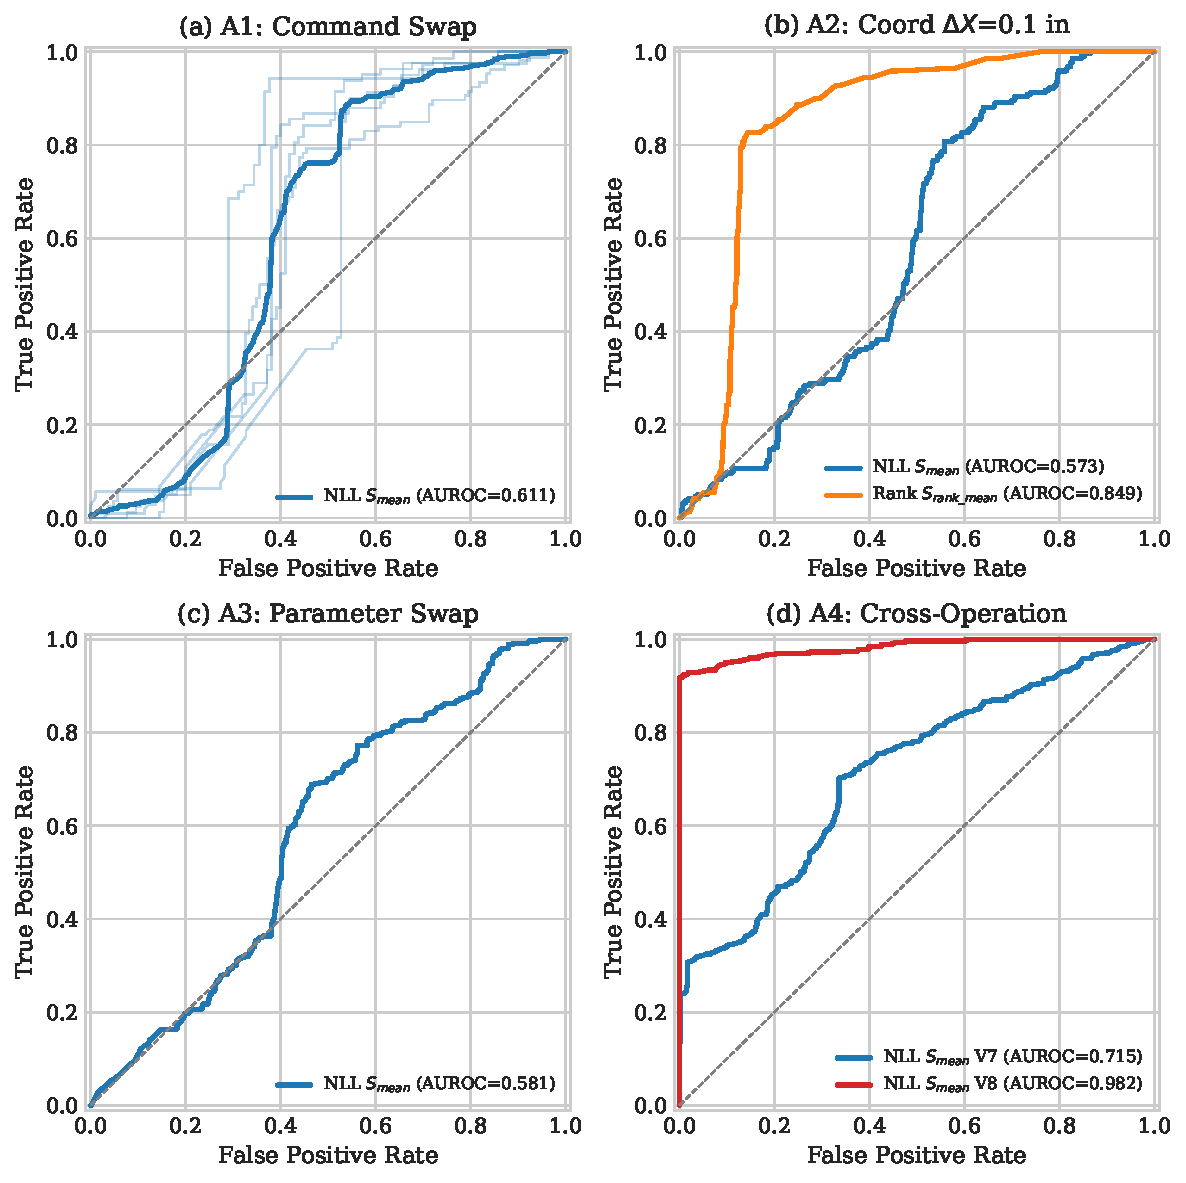
\includegraphics[width=\columnwidth]{figures/roc_curves.pdf}
\caption{ROC curves for four attack types. (a)~A1 command swap: per-fold curves (thin) and mean (thick). (b)~A2 coordinate perturbation ($\delta = 0.1$~in): NLL (blue) vs.\ rank scoring (orange), showing rank's clear advantage. (c)~A3 parameter swap. (d)~A4 cross-operation swap: V7 (blue) vs.\ V8 (red), showing V8's improvement from multi-line context.}
\label{fig:roc_curves}
\end{figure}

\begin{figure}[t]
\centering
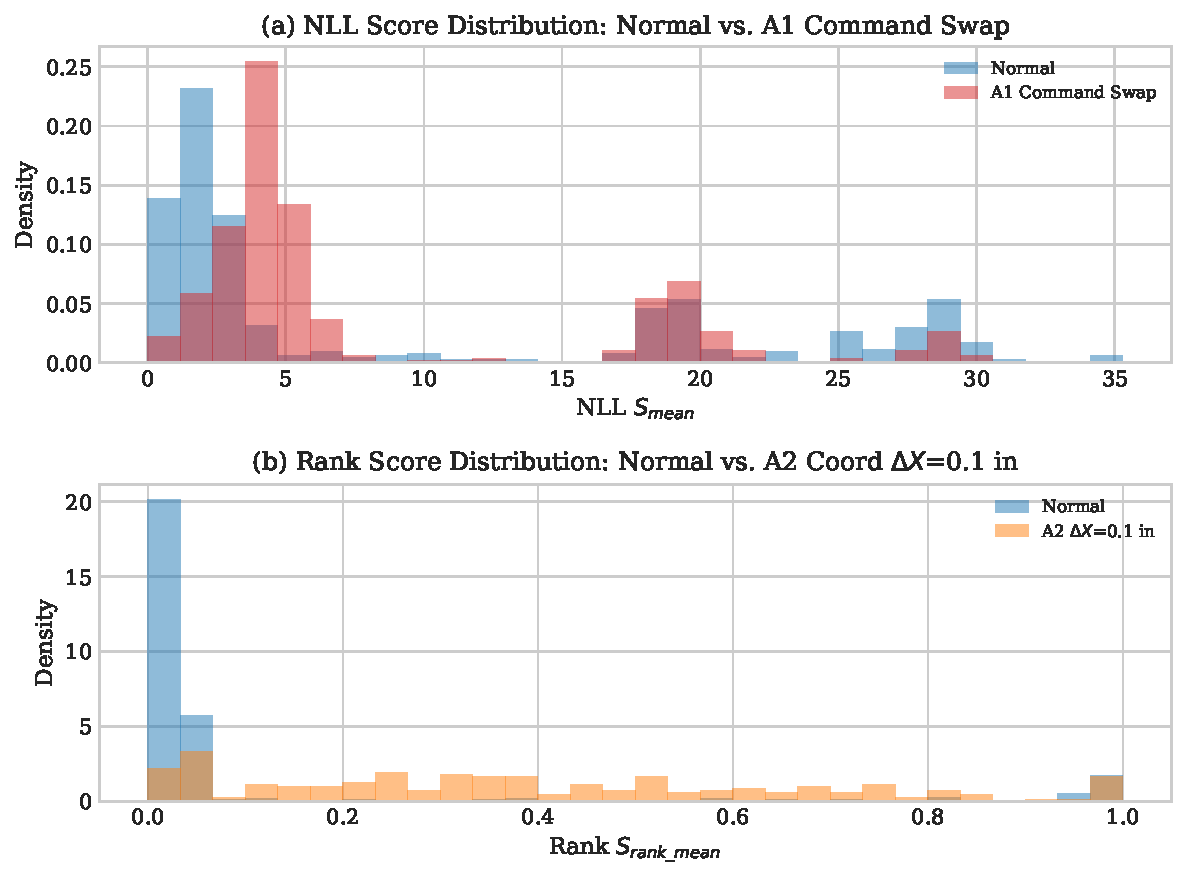
\includegraphics[width=\columnwidth]{figures/score_distributions.pdf}
\caption{Score distributions for normal (blue) vs.\ attacked (red/orange) windows. (a)~NLL $S_{\text{mean}}$: the spread of the normal distribution reflects the per-token confidence gradient (Section~\ref{sec:results_two_populations}). (b)~Rank $S_{\text{rank}}$: clear separation between normal and coordinate-attack windows.}
\label{fig:score_distributions}
\end{figure}

\paragraph{Perturbation-magnitude dependence.}
Larger perturbations are not always easier to detect.
Under V7, $S_{\text{rank}}$ AUROC drops from 0.859 ($\delta = 0.001$) to 0.599 ($\delta = 50$~in) because large perturbations push the axis value into a regime where the decoder's distribution is nearly uniform.
In that regime, both the original and perturbed values become equally implausible.
V8 partially recovers at large $\delta$ ($S_{\max}$ AUROC = 0.797) because multi-line context constrains the plausible coordinate range, so a coordinate far outside the range implied by surrounding lines produces a large $S_{\max}$ value.
Figure~\ref{fig:detection_vs_delta} traces this relationship across five perturbation magnitudes and four scoring methods.

\begin{figure}[t]
\centering
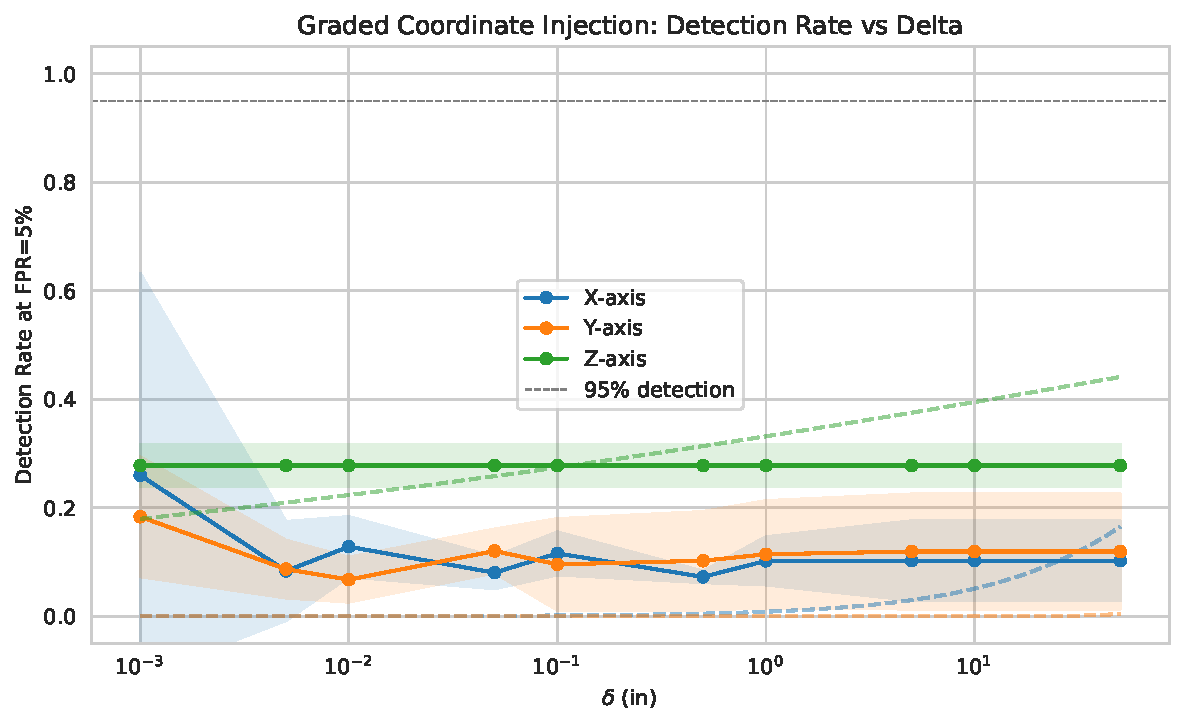
\includegraphics[width=\columnwidth]{figures/detection_vs_delta.pdf}
\caption{Detection AUROC vs.\ perturbation magnitude for X-axis coordinate attacks (A2). V7 rank scoring (orange) dominates at small $\delta$; V8 $S_{\max}$ (red dashed) recovers at large $\delta$ where rank scoring fails. Shaded bands show $\pm$1 std across 5 folds.}
\label{fig:detection_vs_delta}
\end{figure}

\begin{figure}[t]
\centering
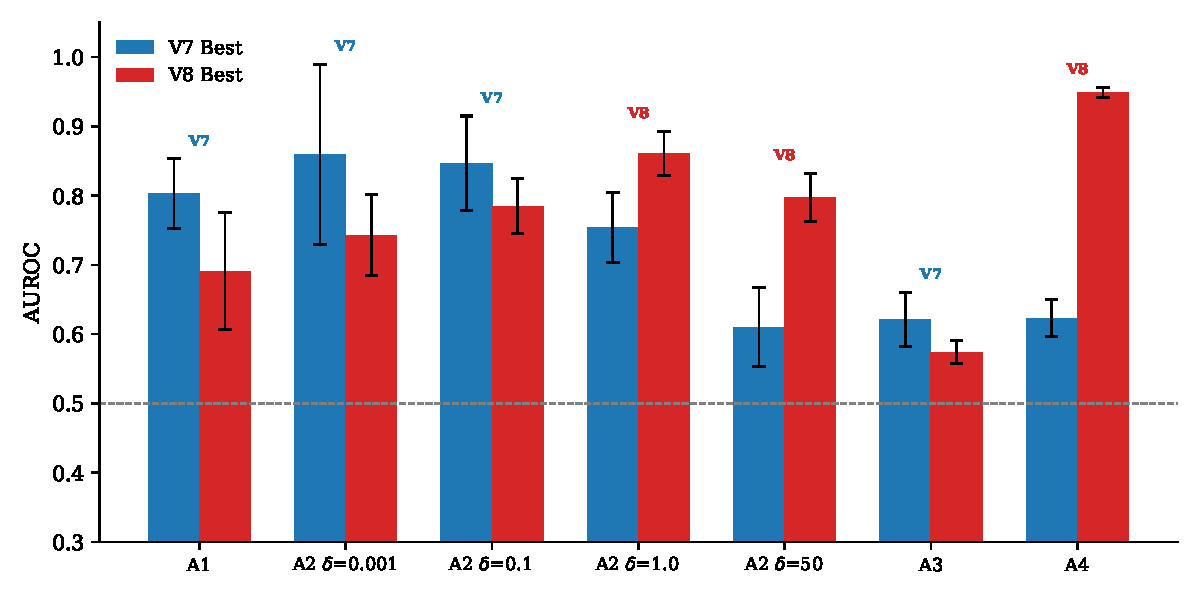
\includegraphics[width=\columnwidth]{figures/v7_v8_comparison.pdf}
\caption{Best AUROC per attack type for V7 (blue) vs.\ V8 (red) decoders. V7 dominates on structural attacks (A1, A3) and small coordinate perturbations; V8 dominates on large perturbations and cross-operation swaps.}
\label{fig:v7_v8_comparison}
\end{figure}

\paragraph{Axis dependence.}
X-axis perturbations are most detectable (V7 AUROC = 0.697 at $\delta = 0.001$), followed by Y (0.640) and Z (0.542).
Z-axis $S_{\text{mean}}$ AUROC is \emph{bit-identical} (0.542) across all ten magnitudes from 0.001 to 50~in.
This exact invariance is a tokenization artifact rather than a detectability plateau.
Z values are sparse in the corpus (depth changes are infrequent), so most Z perturbations round back to the original token and produce no change.
We therefore restrict coordinate-attack claims to the X and Y axes, where the vocabulary is dense enough to realize the requested perturbation.

\subsection{Encoder vs.\ Decoder Detection}
\label{sec:results_enc_dec}

Table~\ref{tab:encoder_vs_decoder} compares encoder-only and decoder-based detection.

\begin{table}[t]
\centering
\caption{Encoder-only vs.\ decoder-based detection on A1 command-swap attacks (mean $\pm$ std across 5 folds). For G-code integrity attacks the sensor window is \emph{identical} between the normal and attacked variant (only the claimed G-code differs), so any method scoring in sensor space yields AUROC = 0.500 by construction. The decoder, which scores the claimed tokens against the reconstruction, is the only method with detection power.}
\label{tab:encoder_vs_decoder}
\begin{tabular}{@{}lcc@{}}
\toprule
Method & AUROC & $\Delta$ vs.\ Decoder V7 \\
\midrule
Encoder DTAE reconstruction\textsuperscript{$\ddagger$} & $0.500$ & $-0.303$ \\
Encoder memory-norm proxy   & $0.500 \pm 0.000$ & $-0.303$ \\
Embedding distance (Mahalanobis)\textsuperscript{$\ddagger$} & $0.500$ & $-0.303$ \\
\midrule
\textbf{Decoder V7 NLL} ($S_{\text{mean}}$)  & $\mathbf{0.803} \pm 0.050$ & --- \\
\bottomrule
\multicolumn{3}{@{}l}{\footnotesize \textsuperscript{$\ddagger$}At chance by construction: the sensor input is unchanged by a G-code-only attack.}
\end{tabular}
\end{table}

Every sensor-space method (DTAE reconstruction error, encoder memory-norm, and Mahalanobis embedding distance) is at chance (AUROC = 0.500) on G-code integrity attacks.
This reflects a structural fact of the threat model rather than a deficiency of those methods.
An A1/A3 attack modifies only the \emph{claimed} G-code and leaves the physical process (and hence every sensor channel) unchanged, so a sensor-only detector receives an identical input for the normal and attacked windows and cannot separate them even in principle (Section~\ref{sec:disc_multiscale}).
The decoder reaches AUROC = $0.803 \pm 0.050$ because it alone compares the claimed token sequence against the sensor-derived reconstruction.

This same property reverses for \emph{physical damage} detection, where the attack \emph{does} alter the sensor signal.
Using the V8 pipeline, the encoder detects damage well, with AUROC = 0.874 (damage vs.\ normal adaptive), 0.949 (face), and 0.703 (pocket).
The decoder is weaker (0.465, 0.747, 0.416) because altered sensors can yield reconstructions that happen to remain consistent with the claimed G-code.
(The shorter V7 pipeline gives weaker, mixed damage AUROCs for both.)
Encoder and decoder thus address complementary threats.
The encoder covers physical-process anomalies that perturb the sensors, and the decoder covers G-code integrity violations that do not.

\subsection{Two-Population Analysis}
\label{sec:results_two_populations}

Per-token analysis of the V7 decoder reveals a \emph{confidence gradient} that explains the aggregate AUROC values.
We partition numeric tokens by the decoder's per-token confidence, defined as the maximum axis-conditional probability $\max_v p(v)$ on normal data (median 0.51), and measure per-token detection AUROC under an adjacent-token (minimum-resolvable) perturbation:

\begin{itemize}
    \item \textbf{Confident tokens} ($\max_v p(v) > 0.5$, 54.3\% of numeric positions): the decoder concentrates probability on a single preferred value, so a perturbation produces a large probability/rank shift. Per-token AUROC = \textbf{0.888}.
    \item \textbf{Low-confidence tokens} ($\max_v p(v) < 0.01$, 2.6\%): probability is spread across candidates, so a one-step perturbation is nearly undetectable. Per-token AUROC = \textbf{0.559}.
    \item The remaining 43.1\% of tokens fall in between (confidence 0.01--0.5).
\end{itemize}

This is a continuum rather than a bimodal split.
The decoder's confidence is bounded away from zero (no numeric token has full-vocabulary $\max_v p(v) < 0.042$), so no genuinely degenerate near-uniform population exists.
Detectability instead rises smoothly with per-token confidence, a consequence of V7's limited single-line context.
Without surrounding lines, many coordinates remain only partially constrained.

Two implications follow:

\begin{enumerate}
    \item \textbf{Aggregate AUROC is a confidence-weighted average.} The reported 0.697 (A2, $\delta = 0.001$, $S_{\text{mean}}$) pools highly detectable confident tokens with near-undetectable low-confidence ones. Rank-based scoring (Section~\ref{sec:rank_score}) recovers much of the lost signal because it is invariant to absolute probability magnitude, lifting AUROC to 0.859 on the same attack.
    \item \textbf{Multi-line context raises confidence.} V8's higher numeric accuracy (43.4\% vs.\ 16.7\%) reflects a larger confident fraction, directly improving coordinate-attack detection.
\end{enumerate}

\subsection{Calibration}
\label{sec:results_calibration}

Table~\ref{tab:calibration} reports ECE before and after temperature scaling for the V7 decoder.

\begin{table}[t]
\centering
\caption{Calibration results for the V7 decoder (mean across 5 folds). Temperature scaling yields only a marginal ECE reduction on the legacy head, the primary head used for anomaly scoring ($0.353 \to 0.309$ at $T = 1.287$); for the V8 decoder the same procedure \emph{increases} ECE (see text). The command head ($T = 1.0$) is already at its optimum.}
\label{tab:calibration}
\begin{tabular}{@{}lcccc@{}}
\toprule
Head & ECE (pre) & ECE (post) & $\Delta$ECE & $T_{\text{opt}}$ \\
\midrule
Legacy       & 0.353 & 0.309 & $-0.044$ & 1.287 \\
Command      & 0.917 & 0.917 & 0.000 & 1.000 \\
Parameter    & 0.813 & 0.813 & 0.000 & 1.000 \\
\bottomrule
\end{tabular}
\end{table}

For the V7 decoder (Table~\ref{tab:calibration}), temperature scaling slightly reduces legacy-head ECE from 0.353 to 0.309 ($T = 1.287$), a marginal improvement.
The effect reverses for V8, where the same $T$ \emph{increases} legacy-head ECE from 0.176 to 0.242.
The command head concentrates on the 6 command classes observed in the corpus (of its ${\sim}30$-token vocabulary) and the parameter head predicts among the 10 observed parameter classes, with highly skewed distributions (G1 accounts for $>$70\% of command tokens).
High ECE in these heads reflects this class imbalance rather than poor probability ordering.
Since anomaly scoring uses NLL (log-probability of the specific target token) rather than calibrated confidence, the miscalibrated bin-level statistics do not affect detection performance.

Because the optimal temperature varies unpredictably across decoders and anomaly scoring relies on NLL rank-ordering rather than calibrated probabilities, we use \emph{uncalibrated} logits for all scoring.

\subsection{Comparison to Sensor-Only Baselines}
\label{sec:results_baselines}

Table~\ref{tab:baselines} compares our reconstruction-mismatch approach against four sensor-only baselines on synthetic G-code attacks.

\begin{table}[t]
\centering
\caption{Baseline comparison on synthetic G-code attacks (AUROC, mean $\pm$ std across 5 folds). Baselines are our own implementations \emph{inspired by} the cited methods, adapted to use all 110 sensor channels rather than each paper's original sensor subset (Kimmell: power only; Coelho: current + vibration). This gives the baselines strictly more information than the original methods. Despite this advantage, sensor-only approaches cannot detect G-code integrity attacks because sensor signals are unchanged by the adversary.}
\label{tab:baselines}
\small
\begin{tabular}{@{}lccc@{}}
\toprule
Method & A1 (cmd swap) & A3 (param swap) & A4 (cross-op) \\
\midrule
Kimmell Energy AE~\cite{kimmell2025} & $0.469 \pm 0.016$ & $0.487 \pm 0.006$ & $0.517 \pm 0.012$ \\
Coelho 1D-CNN~\cite{coelho2024} & $0.528 \pm 0.018$ & $0.563 \pm 0.034$ & $0.535 \pm 0.030$ \\
Isolation Forest & $0.463 \pm 0.013$ & $0.469 \pm 0.013$ & $0.507 \pm 0.011$ \\
One-Class SVM & $0.484 \pm 0.018$ & $0.500 \pm 0.007$ & $0.526 \pm 0.014$ \\
\midrule
\textbf{Ours} (decoder $S_\text{mean}$) & $\mathbf{0.803} \pm 0.050$ & $\mathbf{0.621} \pm 0.039$ & $0.366 \pm 0.039$ \\
\textbf{Ours} (decoder $S_\text{rank}$)\textsuperscript{$\dagger$} & $0.500$ & $0.500$ & $\mathbf{0.623} \pm 0.027$ \\
\bottomrule
\multicolumn{4}{@{}l}{\textsuperscript{$\dagger$}$S_\text{rank}$ scores only numeric tokens; A1/A3 modify non-numeric tokens, yielding 0.500 by design.}
\end{tabular}
\end{table}

On the structural and semantic attacks reported in Table~\ref{tab:baselines} (A1, A3, A4), all four baselines sit near chance (AUROC 0.46--0.56), as expected given that the attack leaves the sensor signals unchanged.
These near-chance values should not be read as an exact 0.500 for \emph{every} attack.
For A2 coordinate perturbations the \emph{unpaired} baselines scatter widely (e.g., at $\delta = 0.001$~in, Coelho 1D-CNN reaches AUROC 0.846 while Isolation Forest falls to 0.128).
These deviations are a \emph{window-selection artifact}.
Only a subset of windows is perturbable at a given $\delta$, and that subset has distinguishable sensor characteristics, so the unpaired baselines discriminate \emph{which windows are attackable} rather than \emph{whether} an attack occurred (the well-below-chance Isolation-Forest value confirms this is not detection).
The paired comparison of Table~\ref{tab:encoder_vs_decoder}, which holds the sensor window fixed, removes this artifact and yields exactly 0.500.
Our reconstruction-mismatch approach is therefore the only method with genuine detection power, because it compares sensor-derived predictions against the claimed G-code rather than scoring sensor windows in isolation.
This advantage comes at higher computational cost (27.2M parameters; measured decoder latency 5.8~ms/window on GPU, 22.3~ms on CPU, vs.\ $<$1~ms for statistical baselines).
The cost is justified because no simpler method can detect G-code integrity attacks at all.

For \emph{physical damage} detection (drive band removed), sensor-only baselines perform comparably, since damage directly alters sensor signals.
One-Class SVM achieves AUROC = $0.769 \pm 0.065$ and Coelho 1D-CNN achieves $0.729 \pm 0.130$.

\subsection{Learned Anomaly Classifier}
\label{sec:results_anomaly_head}

Table~\ref{tab:anomaly_head} presents the XGBoost anomaly classifier trained on 265-dimensional feature vectors combining encoder memory [256], NLL statistics [3], rank scores [2], and per-head entropy [4].

\begin{table}[t]
\centering
\caption{Learned anomaly classifier (XGBoost) vs.\ individual scoring methods (AUROC, mean across 5 folds). The classifier combines encoder memory features [256], NLL statistics [3], rank scores [2], and per-head entropy [4] to learn the mismatch signature. It achieves the highest AUROC on coordinate attacks, reaching 0.962 on A2 with $\delta = 0.001$~in.}
\label{tab:anomaly_head}
\small
\begin{tabular}{@{}lccccc@{}}
\toprule
Attack & NLL & Rank & XGB Head & $\Delta$ vs.\ prev.\ best \\
\midrule
A1 command swap & \textbf{0.803} & 0.500 & 0.754 & $-0.049$ \\
A2 X $\delta{=}0.001$ in & 0.697 & 0.859 & \textbf{0.962} & $+0.103$ \\
A2 X $\delta{=}0.1$ in & 0.676 & 0.847 & \textbf{0.866} & $+0.019$ \\
A2 X $\delta{=}1.0$ in & 0.637 & 0.754 & \textbf{0.771} & $+0.017$ \\
A3 param swap & 0.621 & 0.500 & \textbf{0.656} & $+0.035$ \\
A4 cross-op & 0.366 & 0.623 & \textbf{0.718} & $+0.095$ \\
\bottomrule
\end{tabular}
\end{table}

The XGBoost classifier achieves the highest detection across four of six attack categories.
On small coordinate perturbations (A2, $\delta = 0.001$~in), it reaches AUROC = 0.962, a 10.3 percentage point improvement over rank-based scoring alone.
For cross-operation attacks (A4), it achieves 0.718 versus 0.623 for rank scoring (+9.5~pp).

We attribute the classifier's advantage to its combination of complementary signals: encoder memory captures sensor-level patterns, NLL captures per-token reconstruction quality, and rank scores capture within-axis ordering.
The classifier underperforms only on A1 command swap (0.754 vs.\ NLL's 0.803).
There the raw NLL spike from a single command substitution is already a strong signal, and the classifier's additional features dilute it.

Unlike the unsupervised scoring methods (NLL, rank, embedding distance), the XGBoost classifier requires labeled attack examples during training.
It is therefore a \emph{supervised} detector that cannot generalize to unseen attack types without retraining.
We include it to establish an upper bound on detection performance when attack signatures are known a priori.

For deployment, two modes are available: (1)~\emph{unsupervised mode} using $S_{\text{mean}}$ for structural attacks and $S_{\text{rank}}$ for coordinate attacks, requiring no attack labels; (2)~\emph{supervised mode} using the XGBoost classifier when representative attack examples are available, with raw NLL as a fallback for structural attacks where the classifier underperforms.
We treat the unsupervised path as the deployable system (peak AUROC 0.803 on A1, 0.859 on small coordinate attacks) and the supervised 0.962 strictly as the upper bound established above.

\subsection{Compound Attacks, Significance, and Adaptive Adversaries}
\label{sec:results_revision}

\paragraph{Compound attacks (A9).}
We evaluate a grammar-compliant compound attack that applies both a command swap (A1) and an $X$-coordinate shift ($\delta = 0.1$~in) within the same window.
Detection is \emph{stronger} than for either component alone.
V7 $S_{\text{mean}}$ reaches AUROC = $0.872 \pm 0.039$ (versus 0.803 for A1 and 0.676 for A2 at $\delta = 0.1$ alone) because the two perturbations contribute independent surprise to the short token sequence.

\paragraph{Feed-rate manipulation (A5) is not evaluable on this corpus.}
A5 scales feed-rate ($F$) values.
In our tokenized corpus the feed rate is effectively constant.
The 712-token vocabulary contains a single $F$ value and no spindle-speed ($S$) tokens, and $F$ tokens do not appear in any test window.
Any feed-scaling therefore maps back to the same token, making A5 a no-op.
This is a dataset limitation (constant programmed feed rate), not a limitation of the method, and we report it rather than fabricate a result.

\paragraph{Statistical significance.}
Pairwise AUROC comparisons use the DeLong test with Holm--Bonferroni family-wise correction (Section~\ref{sec:statistical_methods}). The rank-over-NLL advantage on small coordinate attacks is significant at every magnitude tested ($p \leq 1.2\times10^{-5}$ after correction), confirming the effect is not a small-sample artifact.

\paragraph{Adaptive adversary.}
The black-box results above assume a \emph{non-adaptive} attacker that applies a fixed perturbation.
We additionally model a first-order adaptive attacker that, per window, selects the perturbation magnitude ($\delta \geq 0.1$~in, i.e.\ still sabotage-relevant) minimizing the detector's score.
Against the V7 $S_{\max}$ scorer, detection collapses from AUROC = 0.790 (fixed $\delta = 0.1$~in) to \textbf{0.541} (near chance), an evasion drop of 0.249.
An attacker who can probe the detector can therefore largely evade single-score detection by choosing where on the magnitude--detectability curve to operate.
We accordingly frame all detection numbers as detection-under-non-adaptive-attack (Section~\ref{sec:limitations}).

\section{Ablation and Robustness Studies}
\label{sec:ablation}

\subsection{Sensor Modality Importance}
\label{sec:ablation_sensor}

A methodologically valid sensor-modality ablation requires re-encoding each window with the target modality's \emph{input} channels masked and regenerating the encoder memory. The full-feature encoder checkpoint that produced our cached memory is no longer available. A memory-subspace permutation proxy, which perturbs fixed slices of the 256-dimensional \emph{fused} encoder memory, is uninterpretable as modality importance because the fused representation mixes all channels, so no fixed slice corresponds to an identifiable sensor modality. We accordingly do not report per-modality importance rankings, and we caution against drawing modality conclusions from fused-memory perturbations.

This omission is consistent with the central result of Section~\ref{sec:results_enc_dec}. Because sensor-space scores are at chance by construction for G-code integrity attacks, the discriminative signal lies in \emph{token space}, in the decoder's NLL of the claimed program against the sensor-derived reconstruction, rather than in any individual sensor modality. \emph{Which} sensor channels best support the encoder's reconstruction is a property of the encoder, characterized in the companion study~\cite{eacuello2026decoder}, rather than of attack detection.

\subsection{Partial Sensor Failure Robustness}
\label{sec:ablation_partial}

We simulate sensor board failure by zeroing out channels for one or more boards at test time without retraining.
Table~\ref{tab:sensor_failure} reports single- and two-board failure scenarios.

\begin{table}[t]
\centering
\caption{Detection performance under simulated sensor board failure (A1 command swap, V7 $S_{\text{mean}}$, mean across 5 folds). Boards are zeroed at test time without retraining. The system degrades gracefully: worst single-board removal costs only 1.4~pp.}
\label{tab:sensor_failure}
\begin{tabular}{@{}lcc@{}}
\toprule
Failure Scenario & Boards & AUROC (V7, A1) \\
\midrule
Full system              & 0 & 0.803 \\
Best single-board-out    & 1 (Bd.\ 0) & 0.825 \\
Worst single-board-out   & 1 (Bd.\ 3) & 0.789 \\
Second-worst single      & 1 (Bd.\ 5) & 0.796 \\
Worst two-boards-out     & 2 (Bd.\ 2+3) & 0.782 \\
Best two-boards-out      & 2 (Bd.\ 0+4) & 0.859 \\
\bottomrule
\end{tabular}
\end{table}

The system degrades gracefully under simulated board failure.
Worst-case single-board removal reduces AUROC by only 0.014 (Board~3, 0.803 to 0.789), and worst-case two-board removal yields 0.782 ($-0.021$).
Some removals \emph{improve} performance (Board~0, AUROC = 0.825), suggesting certain boards contribute noisy signals not fully compensated by modality dropout.
We attribute the graceful degradation to modality-dropout training and to measurement redundancy across six overlapping sensor positions.

\subsection{Cross-Condition Generalization}
\label{sec:ablation_crosscondition}

We evaluate whether anomaly score distributions are consistent across machining conditions (air-cut, active-cut, damage-condition), because threshold transferability across conditions depends on this consistency.
Table~\ref{tab:cross_condition} summarizes the results.

\begin{table}[t]
\centering
\caption{Cross-condition score distribution analysis (V8 $S_{\text{mean}}$ on normal data). The Kolmogorov--Smirnov (KS) statistic and Cohen's $d$ quantify the distributional shift between conditions. Air-cut vs.\ active-cut shows the largest shift ($d = -0.70$), indicating that a threshold calibrated on one condition may not transfer to the other. The shorter-context V7 decoder shows the same qualitative ordering but smaller, non-significant shifts (see text).}
\label{tab:cross_condition}
\begin{tabular}{@{}lccc@{}}
\toprule
Condition Pair & KS Statistic & Cohen's $d$ & $p$-value \\
\midrule
Air-cut vs.\ active-cut   & 0.608 & $-0.702$ & $< 10^{-6}$ \\
Air-cut vs.\ damage       & 0.624 & $-0.586$ & $5.2 \times 10^{-4}$ \\
Active-cut vs.\ damage    & 0.267 & $+0.070$ & 0.385 \\
\bottomrule
\end{tabular}
\end{table}

For the V8 decoder, the largest shift occurs between air-cut and active-cut windows ($d = -0.70$, $p < 10^{-6}$).
Air-cut windows contain simple, predictable G-code (G0 rapid moves) and yield low NLL, while active-cut windows contain variable coordinates and yield higher NLL.
A threshold calibrated on one condition would therefore produce mismatched false positive rates on the other.
The active-cut and damage distributions, in contrast, are statistically indistinguishable ($d = +0.07$, $p = 0.385$), so a threshold calibrated on active cutting transfers to the damage condition.

The shorter-context V7 decoder exhibits the same ordering but weaker, statistically non-significant shifts (air-cut vs.\ active-cut KS = 0.327, $p = 0.099$, $d = -0.50$; air-cut vs.\ damage KS = 0.476, $p = 0.108$; active-cut vs.\ damage KS = 0.436, $p = 0.166$).
V7's three-token windows carry less condition-discriminating information than V8's multi-line windows.
Threshold transferability is thus a concern primarily for the multi-line decoder.

\subsection{Window Position Confound}
\label{sec:ablation_position}

Removing window position encoding from the decoder degrades A1 AUROC from $0.803 \pm 0.050$ to $0.638 \pm 0.030$ ($-16.5$~pp).
Position information thus contributes substantially to detection.
CNC programs have deterministic structure, with predictable setup commands early and retract sequences late, which a position-aware detector leverages.
The no-position ablation nevertheless remains well above chance ($0.638 \pm 0.030$ vs.\ 0.500), confirming genuine sensor-to-G-code reconstruction signal beyond program-position priors.

\paragraph{NLL variation with position.}
NLL varies systematically with window position.
It is low during the predictable early-program setup and late-program shutdown and high during mid-program active cutting.
A position-normalized scoring approach (subtracting position-specific mean NLL) would mitigate this, but insufficient windows per position bin in our dataset prevent reliable estimation.

\subsection{Feature Configuration Ablation}
\label{sec:ablation_features}

Table~\ref{tab:feature_config} compares three feature configurations.

\begin{table}[t]
\centering
\caption{Detection performance across feature configurations (A1 command swap, V7 $S_{\text{mean}}$). AUROC varies by less than 0.02 across configurations between the full (f110) and minimal (f56) feature sets. The minimal configuration actually achieves the highest AUROC, likely due to reduced noise from uninformative channels.}
\label{tab:feature_config}
\begin{tabular}{@{}lccc@{}}
\toprule
Configuration & Channels & AUROC & $\Delta$ vs.\ f110 \\
\midrule
f110 (full)       & 110 & 0.803 $\pm$ 0.050 & --- \\
f98 (no redundant) & 98  & 0.796 $\pm$ 0.052 & $-0.007$ \\
f56 (minimal)      & 56  & 0.812 $\pm$ 0.041 & $+0.009$ \\
\bottomrule
\end{tabular}
\end{table}

AUROC varies by less than 0.02 across all configurations.
The minimal f56 set (accelerometers, gyroscopes, audio, electrical) slightly exceeds f110, though the difference is not statistically significant.
The core physical modalities suffice.
Additional channels (environmental, color, magnetometer) may introduce marginal noise.
The f98 configuration offers a practical deployment compromise, reducing dimensionality by 11\% with negligible performance impact ($-0.007$).

\subsection{Leave-One-Class-Out (LOCO) Analysis}
\label{sec:ablation_loco}

LOCO retrains the decoder on 8 of 9 classes and scores the held-out class as anomalous, testing detection of entirely novel operation types.

\begin{table}[t]
\centering
\caption{Leave-one-class-out AUROC (mean across 5 CV folds). Face milling classes are the most detectable as novel ($> 0.73$), while pocket and adaptive classes are poorly detected ($< 0.47$), reflecting their sensor-signature similarity to the training distribution.}
\label{tab:loco}
\begin{tabular}{@{}lcc@{}}
\toprule
Held-Out Class & AUROC & Cohen's $d$ \\
\midrule
face            & 0.852 & $+1.88$ \\
face150025      & 0.735 & $+0.79$ \\
pocket          & 0.323 & $-0.64$ \\
pocket150025    & 0.472 & $-0.22$ \\
adaptive        & 0.428 & $-0.31$ \\
adaptive150025  & 0.409 & $-0.30$ \\
\bottomrule
\multicolumn{3}{@{}p{0.80\columnwidth}}{\footnotesize The six non-damage operation classes are shown; the three damaged-spindle classes are omitted here (their LOCO AUROCs are 0.49--0.64: damageface 0.637, damagepocket 0.567, damageadaptive 0.488).}
\end{tabular}
\end{table}

Performance is highly class-dependent.
Face milling is reliably detected as novel (AUROC = 0.852, $d = 1.88$), indicating distinctive signatures that the decoder cannot reconstruct when trained on the other classes.
Pocket and adaptive classes are poorly detected (AUROC = 0.323--0.472), consistent with sensor signatures that overlap the remaining training classes.
LOCO-style detection is therefore unreliable in general.
The reconstruction-mismatch framework is better suited to detecting modifications within known programs (A1--A4) than to detecting unknown programs.

\section{Discussion}
\label{sec:discussion}

\subsection{Error Taxonomy and Failure Modes}
\label{sec:disc_errors}

Systematic error analysis (Experiment~9) reveals two distinct failure modes.

\paragraph{False positives.}
False positives cluster in three categories: (1)~windows containing rare but legitimate G-code patterns---unusual coordinates near workpiece boundaries, infrequent M-codes, and cutting/rapid-traverse transitions---that are underrepresented in training data; (2)~program-boundary windows (startup/shutdown sequences) where the decoder predicts with moderate but imperfect confidence; and (3)~tool-change sequences (M6--G43--G0), where the decoder assigns $p \approx 0.15$ to M6 versus $p \approx 0.45$ to the more common G1, producing NLL of 4.2 versus a normal-window mean of 3.1~nats.

For the V7 decoder, reconstruction errors concentrate in the \emph{middle} of each program (early 17.5\%, middle 50.8\%, late 31.7\%; Cram\'er's $V = 0.353$, $\chi^2$ significant across folds), where active-cutting coordinate density is highest, and are sparsest in the predictable early-program setup. The position--error-type association is statistically significant, not uniform.

\paragraph{False negatives.}
Two scenarios produce the most challenging false negatives.
Coordinate perturbations (A2) that modify low-confidence numeric tokens produce small $\Delta$NLL---insufficient for reliable NLL-based detection (rank scoring partially recovers these; Section~\ref{sec:results_two_populations}).
Parameter substitutions (A3) are the hardest attack type overall (best AUROC = 0.621) because swapping parameter letters preserves the numeric value, and the V7 decoder's high parameter-token error rate (45.3\%) means substituted parameters often receive non-negligible probability.

\subsection{Scoring Method Complementarity}
\label{sec:disc_multiscale}

Three forms of complementarity shape the detection landscape.

\paragraph{V7/V8 scale complementarity.}
Short-context decoding (V7) localizes per-token anomalies; multi-line decoding (V8) captures sequential patterns.
This parallels the resolution trade-off in signal processing and motivates running both decoders in parallel.

\paragraph{NLL/rank complementarity.}
For uncertain numeric tokens, the decoder assigns negligible probability to all candidates ($p = 0.003$ original vs.\ $p = 0.002$ perturbed, $\Delta$NLL = 0.41~nats---within noise).
Rank scoring bypasses this by detecting \emph{ordinal} shifts: if the original value sits at rank~45 and the perturbed value at rank~120, the normalized difference of 0.105 is detectable even when absolute probabilities are negligible.
Conversely, rank scoring fails on parameter substitutions (A3 AUROC = 0.500) because it only operates on numeric tokens.
A grid-searched ensemble over NLL, rank, and Mahalanobis distance matches the best individual scorer per attack type (AUROC = 0.859 on A2, 0.647 on A4) but does not exceed it; a combined logistic regression yields AUROC = $0.663 \pm 0.020$, confirming that no single linear combination dominates. We note that these grid-searched weights are tuned on the evaluation windows and so represent an \emph{in-sample upper bound}; the per-attack-type routing of Eq.~\ref{eq:s_hybrid} is the deployable alternative.

\paragraph{Continuous vs.\ discrete scoring.}
Replacing continuous NLL with binary argmax comparison degrades detection in most settings because it discards graded confidence.
The exception is V7 on A4 (argmax AUROC = 0.629 vs.\ NLL = 0.366), where discrete disagreements avoid dilution by uncertain tokens---further evidence that the confident/uncertain token split governs detection behavior.

\subsection{Temporal Detection via CUSUM}
\label{sec:disc_cusum}

CUSUM control charts~\cite{page1954cusum} applied to the NLL time series across consecutive windows (Experiment~18) achieve a mean detection rate of 65.9\% ($\pm$ 13.0\%) with detection latency of 1.3 windows.
The 38.6\% false alarm rate renders the current CUSUM implementation impractical for deployment. This high rate stems from per-window NLL variance, which causes frequent threshold crossings even under normal operation. Practical deployment would require either (a) substantially longer averaging windows, (b) adaptive thresholds conditioned on operation type, or (c) a different temporal aggregation strategy.

\subsection{Cost-Benefit Analysis for Deployment}
\label{sec:disc_cost}

The complete sensor instrumentation costs \$492 (Table~\ref{tab:sensor_cost})---of which the six Arduino boards account for \$198 (\$33 each) and the DAQ, aggregator, and cabling the remainder---representing 0.1--1.0\% of a typical production CNC machine (\$50K--\$500K) and amortized over a 10--20 year operational lifetime.
Measured decoder inference is 5.8~ms per window on an RTX~A6000 GPU (11{,}000$\times$ faster than the 64-second window) and 22.3~ms on an Intel Xeon CPU (2{,}870$\times$ real-time), exclusive of sensor encoding---a negligible duty cycle either way.

To illustrate the economic case, we construct a simplified cost model with the parameters used in our analysis: sensor hardware cost of \$492, 5000 windows/day, investigation cost of \$50/alarm, attack probability of $10^{-3}$/day, and \$10K damage per undetected attack. Under these assumptions---which we emphasize are illustrative, not empirical---the system yields positive expected value. Real deployment would require facility-specific calibration of attack probability and damage cost parameters.

\subsection{Comparison to Prior Work}
\label{sec:disc_comparison}

No standardized benchmark exists for CNC attack detection, precluding direct quantitative comparison.
Table~\ref{tab:comparison} provides a qualitative comparison.

\begin{table}[t]
\centering
\caption{Qualitative comparison with prior CNC attack detection methods. Our approach is the only method that performs integrity verification (sensor--G-code consistency) rather than fault detection or classification. ``Unsupervised w.r.t.\ attacks'' means the model is trained only on normal data and does not require labeled attack examples.}
\label{tab:comparison}
\small
\begin{tabular}{@{}p{2.5cm}p{2cm}p{2.5cm}p{1.5cm}p{2cm}@{}}
\toprule
Method & Sensor Input & Approach & Attack Types & Requires Attack Labels \\
\midrule
Kimmell~\cite{kimmell2025} & Power & Energy profiling & Gross toolpath changes & No \\
Coelho~\cite{coelho2024} & Vibration & 1D-CNN classifier & Known faults & Yes \\
Moore~\cite{moore2017power} & Power & Statistical process control & Power anomalies & No \\
Chhetri~\cite{chhetri2016kcad} & Kinetic & Kinetic fingerprinting & Geometry deviation & No \\
\midrule
\textbf{This work} & \textbf{Multi-modal (110 ch.)} & \textbf{Reconstruction mismatch} & \textbf{G-code modifications (A1--A4)} & \textbf{No} \\
\bottomrule
\end{tabular}
\end{table}

Our approach differs from prior methods in three respects: (1)~it performs \emph{integrity verification} (sensor vs.\ claimed G-code) rather than fault detection from a statistical baseline; (2)~it uses \emph{multi-modal} input (110 channels, 7 modality groups); and (3)~it requires no labeled attack examples.
The trade-off is complexity: our system needs 6 sensor boards and a trained deep learning model, whereas power monitoring~\cite{kimmell2025,moore2017power} needs a single sensor and simple statistical rules.
This complexity is justified when the threat model includes subtle attacks ($\delta = 0.001$~mm coordinate perturbations) invisible to energy monitoring.

\subsection{Analytical vs.\ Experimental Detection Rates}
\label{sec:disc_gap}

Prior work on this dataset~\cite{eacuello2026decoder} reported analytical detection rates of 98.7\% for command injection and 97.8\% for structural attacks by reinterpreting decoder reconstruction accuracy as a detection metric.
Our experimental evaluation---which generates actual attack variants, computes per-token NLL, and evaluates detection at controlled false-positive rates---yields substantially lower AUROCs (0.803 for A1 command swap, 0.621 for A3 parameter substitution).

Three factors explain the gap.
First, the analytical approach assumes that any reconstruction error is a detection signal; experimentally, reconstruction errors on \emph{normal} windows produce false positives that degrade AUROC.
Second, the confidence gradient (Section~\ref{sec:results_two_populations}) means a large share of numeric tokens are low-confidence and contribute noise rather than signal to the mean NLL, diluting detection power.
Third, the analytical rates count per-token accuracy rather than per-window detection decisions, which is a more permissive metric.

This gap underscores the importance of experimental evaluation: analytical detection rates can substantially overstate operational performance.

\section{Limitations}
\label{sec:limitations}

\begin{enumerate}
    \item \textbf{Single machine and material.}
    All experiments use a single Bantam Tools desktop CNC mill (air-cut runs and dry UHMW-PE active cuts).
    Industrial CNC machines vary widely in kinematics, controllers, and power levels.
    Metals produce different sensor signatures than UHMW-PE.
    The reconstruction-mismatch principle should generalize, but the specific AUROCs reported here require empirical validation on other platforms and materials.

    \item \textbf{Synthetic, non-adaptive attacks; integrity-check threat model.}
    All attacks are synthetically generated by modifying G-code tokens post-alignment.
    The headline AUROCs assume a \emph{non-adaptive} attacker.
    A first-order adaptive attacker that selects, per window, the (still sabotage-relevant) perturbation minimizing the detector score drops single-score detection to near chance (AUROC = 0.54; Section~\ref{sec:results_revision}).
    Robust detection against such an adversary is unsolved.
    The evaluation further assumes the sensors reflect the \emph{original} program while the claimed G-code is the attacker's.
    This assumption fits post-transmission/at-rest integrity verification against an authenticated original-run trace.
    It does \emph{not} cover attacks that modify G-code \emph{before} execution so that the sensors reflect the tampered process (the canonical dr0wned/Sturm scenario), a regime this method cannot detect.

    \item \textbf{Small dataset.}
    The 120-file dataset (${\sim}545$ sensor windows) limits statistical power.
    Several attack-type/method combinations have confidence intervals encompassing chance (e.g., V7 $S_{\text{mean}}$ on A2 at $\delta = 0.001$~in: AUROC = $0.697 \pm 0.151$).
    The damage-condition classes (4--5 files each) are particularly underrepresented.

    \item \textbf{Known toolpath vocabulary.}
    The system is trained on a fixed set of 9 toolpath classes with a 712-token vocabulary.
    Novel G-code programs using different commands or coordinate ranges may trigger false positives.
    Introducing new programs therefore requires periodic retraining.

    \item \textbf{Sensor trustworthiness assumption.}
    The threat model assumes sensor signals cannot be spoofed (Section~\ref{sec:adversary}).
    An attacker who simultaneously modifies G-code and injects false sensor data (via physical tampering, bus interception, or software compromise) could evade detection entirely.
    The assumption holds for hardwired sensors with shielded cables and dedicated data paths, but breaks for wireless or network-accessible sensor interfaces.
    Mitigation requires hardware-level tamper protection (secure enclaves, hardware attestation) for the sensor subsystem.

    \item \textbf{Offline evaluation only.}
    All experiments run in batch mode.
    Real-time deployment introduces latency constraints, windowing edge effects, online threshold adaptation, and CNC controller integration, none of which are evaluated here.
    The measured 5.8~ms/window (GPU) decoder inference latency suggests computational feasibility.

    \item \textbf{Binary detection scope.}
    The system produces a binary normal/anomalous decision without diagnosing attack type, identifying modified parameters, or recommending corrective action.
    Attack diagnosis would require labeled attack examples or interpretability methods tracing anomaly scores to specific token positions.

    \item \textbf{Supervised anomaly classifier.}
    The XGBoost anomaly classifier (Section~\ref{sec:results_anomaly_head}) uses supervised training with labeled attacks.
    Its applicability is therefore limited to attack types seen during training.
\end{enumerate}

\section{Conclusion}
\label{sec:conclusion}

We presented a multi-scale sensor-to-G-code reconstruction mismatch framework for detecting adversarial modifications to CNC machining programs.
An autoregressive decoder reconstructs the G-code token sequence that should have produced the observed multi-modal sensor signals; anomalies manifest as elevated reconstruction error when the claimed G-code is inconsistent with the physical process.

No single decoder configuration or scoring method dominates all attack types.
Short-context decoding (V7) achieves strong structural-attack detection through concentrated per-token probability mass, while multi-line decoding (V8) captures sequential consistency needed for semantic attacks.
Rank-based scoring recovers coordinate-perturbation detection where NLL fails, by exploiting relative probability ordering rather than absolute likelihoods.
The per-token confidence gradient of autoregressive G-code prediction---confident numeric tokens (54\% of positions, per-token AUROC = 0.89) versus low-confidence tokens (per-token AUROC near chance)---is the fundamental factor governing coordinate-attack detection and explains why multi-line context, which raises per-token confidence, improves it.

The system is robust to sensor dropout (worst single-board-out AUROC = 0.789), stable across feature configurations (56--110 channels, AUROC variation $< 0.02$), and deployable at low cost (\$492 sensor hardware; measured decoder inference 5.8~ms/window on GPU, 22.3~ms on CPU).
Several negative results constrain the design space: multi-head disagreement scoring provides no signal (AUROC $\approx$ 0.500), embedding-distance methods are blind to token-level attacks, temperature-scaling calibration degrades ECE, and CUSUM achieves only 65.9\% detection at a 38.6\% false alarm rate.

Future work should address five priorities:
\begin{enumerate}
    \item \textbf{Real-time streaming deployment} with position-normalized scoring and CNC controller integration for automatic process halt.
    \item \textbf{Multi-machine and multi-material generalization} on production-grade machines cutting metals, using transfer learning to reduce retraining costs.
    \item \textbf{Attack diagnosis} beyond binary detection, tracing anomaly scores to specific token positions with estimated modification type and magnitude.
    \item \textbf{Defenses against adaptive adversaries.} Our first-order adaptive attacker already nearly evades single-score detection (AUROC $\to$ 0.54); robust detection will require score ensembling, randomized thresholds, or detectors that bound the worst-case perturbation rather than the average case.
    \item \textbf{Sensor integrity assurance} via hardware attestation and cryptographic authentication to prevent sensor spoofing.
\end{enumerate}

The reconstruction-mismatch paradigm---learning the inverse mapping from physical observations to commands and flagging discrepancies---generalizes beyond CNC machining to any cyber-physical system where a digital program controls a physical process (3D printers, robotic welders, semiconductor fabrication, chemical process controllers).
The key requirement is a sensor suite capturing sufficient physical information to constrain command-sequence reconstruction, a condition increasingly met as Industry~4.0 instrumentation becomes standard.

\section*{Reproducibility}
All training scripts, evaluation code, and experiment configurations will be made available upon publication.
The dataset consists of sensor recordings from a Bantam Tools Desktop CNC milling machine; data sharing is subject to institutional approval.
All reported results use 5-fold cross-validation with file-level stratified splits to prevent data leakage.
Attacks are generated deterministically (seed = 42).
Per-fold results are provided in the supplementary material.


\vspace{6pt}

\authorcontributions{Conceptualization, S.S.E. and R.S.P.; methodology, S.S.E.; software, S.S.E.; validation, S.S.E.; formal analysis, S.S.E.; investigation, S.S.E.; resources, M.S.S.; data curation, S.S.E. and R.S.P.; writing---original draft, S.S.E.; writing---review \& editing, R.S.P. and M.S.S.; visualization, S.S.E.; supervision, R.S.P. and M.S.S.; project administration, R.S.P. All authors have read and agreed to the published version of the manuscript.}

\funding{This material is based upon work partially supported by the Office of Naval Research (ONR) under Contract no. N000142412129.}

\acknowledgments{This material is based upon work partially supported by the Office of Naval Research (ONR) under Contract no. N000142412129. Any opinions, findings, and conclusions or recommendations expressed in this material are those of the author(s) and do not necessarily reflect the view of the ONR. The authors thank the Department of Industrial Systems Engineering and the College of Engineering at the University of Rhode Island for laboratory facilities and computational resources.}

\conflictsofinterest{The authors declare no conflict of interest.}

\newcommand{\dataavailabilitytext}{The sensor datasets and analysis code generated during this study are available from the corresponding author upon reasonable request and at \url{https://github.com/stephenseacuello/gcode_fingerprinting}.}
\ifdefined\dataavailability
  \dataavailability{\dataavailabilitytext}
\else
  \noindent\textbf{Data Availability Statement:} \dataavailabilitytext
\fi

\appendix
\section{Per-Fold Cross-Validation Results}
\label{app:perfold}

Tables~\ref{tab:perfold_v7_nll} and~\ref{tab:perfold_v8_training} report per-fold results for the V7 and V8 decoders, respectively, documenting the fold-to-fold variability underlying the mean AUROC values reported in the main text.

\begin{table}[ht]
\centering
\caption{V7 decoder per-fold AUROC for selected attack types and scoring methods. Fold-to-fold variation is modest for A1 (range = 0.154 for $S_{\text{mean}}$) but substantial for A2 with small $\delta$ (range = 0.431), reflecting the high sensitivity to the specific files in each fold's test set.}
\label{tab:perfold_v7_nll}
\small
\begin{tabular}{@{}lcccccc@{}}
\toprule
Attack / Method & Fold 1 & Fold 2 & Fold 3 & Fold 4 & Fold 5 & Mean \\
\midrule
\multicolumn{7}{@{}l}{\textit{A1 Command Swap --- $S_{\text{mean}}$}} \\
 & 0.726 & 0.823 & 0.800 & 0.787 & 0.880 & 0.803 \\
\multicolumn{7}{@{}l}{\textit{A2 X $\delta$=0.001 --- $S_{\text{mean}}$}} \\
 & 0.984 & 0.653 & 0.604 & 0.688 & 0.554 & 0.697 \\
\multicolumn{7}{@{}l}{\textit{A2 X $\delta$=0.001 --- $S_{\max}$}} \\
 & 0.875 & 0.656 & 0.719 & 0.891 & 0.570 & 0.742 \\
\multicolumn{7}{@{}l}{\textit{A3 Parameter Swap --- $S_{\text{mean}}$}} \\
 & 0.642 & 0.553 & 0.603 & 0.648 & 0.658 & 0.621 \\
\multicolumn{7}{@{}l}{\textit{A4 Cross-Operation --- $S_{\text{mean}}$}} \\
 & 0.427 & 0.343 & 0.320 & 0.393 & 0.346 & 0.366 \\
\bottomrule
\end{tabular}
\end{table}

\begin{table}[ht]
\centering
\caption{V8 decoder reconstruction accuracy per fold. Fold-to-fold variation is modest for token accuracy (range = 3.1~pp) and numeric accuracy (range = 3.4~pp), but wider for command accuracy (range = 8.2~pp), reflecting sensitivity to the operation-class composition of each fold's training set.}
\label{tab:perfold_v8_training}
\begin{tabular}{@{}lccc@{}}
\toprule
Fold & Token Acc.\ (\%) & Numeric Acc.\ (\%) & Command Acc.\ (\%) \\
\midrule
1 & 65.6 & 42.6 & 84.1 \\
2 & 66.9 & 42.2 & 89.5 \\
3 & 66.7 & 43.1 & 90.7 \\
4 & 67.9 & 43.7 & 87.0 \\
5 & 68.7 & 45.6 & 92.3 \\
\midrule
\textbf{Mean} & \textbf{67.2} & \textbf{43.4} & \textbf{88.7} \\
\bottomrule
\end{tabular}
\end{table}

Fold-to-fold variation differs by attack type.
For A1 command swap ($S_{\text{mean}}$), AUROC ranges from 0.726 to 0.880 (range = 0.154), and the lowest fold (Fold~1) remains well above chance.
For A2 X $\delta = 0.001$ ($S_{\text{mean}}$), the range is much wider (0.554 to 0.984).
Fold~1 achieves near-perfect detection (0.984), while Fold~5 is near chance (0.554).
We attribute this variability to the composition of each fold's test set.
Files differ in their share of confident numeric tokens, the population with the highest per-token detectability.
With only $\sim$110 windows per fold, the confident/uncertain ratio can vary between folds.

\section{Vocabulary Structure}
\label{app:vocab}

The G-code vocabulary comprises 712 tokens organized into four semantic categories.
Table~\ref{tab:vocab_structure} provides the breakdown.

\begin{table}[ht]
\centering
\caption{Vocabulary composition (712 tokens total). The multi-head decoder structure assigns each token to one semantic category, enabling fine-grained anomaly attribution.}
\label{tab:vocab_structure}
\begin{tabular}{@{}lrl@{}}
\toprule
Category & Count & Examples \\
\midrule
Special tokens & 5 & PAD, BOS, EOS, UNK, SEP \\
Command tokens & $\sim$30 & G0, G1, G2, G3, M3, M5, M6, M30 \\
Parameter tokens & $\sim$10 & X, Y, Z, F, S, R, I, J, K \\
Numeric tokens & $\sim$667 & \texttt{NUM\_X\_1492}, \texttt{NUM\_Y\_0175}, \\
& & \texttt{NUM\_Z\_0600}, \texttt{NUM\_F\_2000} \\
\bottomrule
\end{tabular}
\end{table}

The multi-head output structure decouples these categories.
The type head selects among \{command, parameter, numeric, special\}, and the category-specific downstream heads predict within each category.
This factored structure reduces the effective vocabulary size per head; the command head, for example, predicts over $\sim$30 candidates rather than 712.
It also enables fine-grained anomaly attribution, because the per-head NLL breakdown indicates which token field is anomalous when the anomaly score is elevated.

\paragraph{Numeric tokenization.}
Numeric values (e.g., the coordinate X3.2750) are decomposed digit-by-digit using the \texttt{DigitByDigitValueHead}.
Each numeric token is decomposed into:
\begin{enumerate}
    \item A sign token ($+$ or $-$)
    \item Up to 4 integer digit tokens (hundreds, tens, ones, and a leading-zero position)
    \item A decimal point token
    \item Up to 4 decimal digit tokens (tenths, hundredths, thousandths, ten-thousandths)
\end{enumerate}
Each numeric token is represented by a sign position plus 6 digit positions, yielding 7 predictions per numeric value.
The digit-by-digit approach avoids the combinatorial explosion of discretizing continuous axis values into fixed bins.
Covering the machine's X-axis travel ($\approx$5.5~in) at the tokenizer's $0.001$~in grid would require $\sim$5{,}500 bins in a direct discretization scheme, compared to approximately 30 token types in the digit-by-digit scheme (10 digits + sign + decimal point, used combinatorially).

% Scoring method implementation details moved to supplementary material.

\section{Error Case Analysis}
\label{app:errors}

Three cases illustrate detection outcomes: a true positive, a false positive, and a false negative.

\paragraph{Illustrative true positive (A1 command swap).}
A sensor window during active face-milling contains the normal G-code sequence: G1 X-10.500 Y5.250 F200.
The decoder assigns $p = 0.72$ to G1 (the correct command) and $p = 0.01$ to G0 (the attacker's substitution).
The per-token NLL is 0.33 nats for the normal token and 4.61 nats for the attacked token, a $14\times$ increase.
The attacked window's $S_{\text{mean}}$ is 2.89 nats versus 1.47 nats for the normal window, well above typical detection thresholds.
This attack is highly detectable because the decoder has learned that G1 (feed-rate interpolation) is the expected motion command during active cutting and that G0 (rapid traverse) is anomalous in this context.

\paragraph{Illustrative false positive (tool-change sequence).}
A window during a tool-change sequence contains M6 (tool change) followed by G43 (tool-length compensation) and G0 (rapid positioning).
The M6 command occurs in fewer than 2\% of training windows, so the decoder assigns only $p \approx 0.15$ to M6 while assigning $p \approx 0.45$ to the more common G1.
This yields $S_{\text{mean}} = 4.2$ nats against a normal-window mean of 3.1 nats, triggering a false alarm at typical detection thresholds.
The false positive arises because rare but legitimate G-code patterns are underrepresented in training, not because the reconstruction is in error.
The decoder correctly identifies M6 as less probable than G1; the ranking is technically accurate but operationally unhelpful.

\paragraph{Illustrative false negative (A2 coordinate perturbation in uncertain regime).}
A coordinate perturbation of $\delta = 0.001$~in on an X-axis value (X3.2750 $\to$ X3.2760, one tokenizer grid step) falls in the decoder's low-confidence regime.
The decoder assigns $p = 0.003$ to the original value and $p = 0.002$ to the perturbed value, yielding $\Delta$NLL $= -\log(0.002) - (-\log(0.003)) = 0.41$ nats.
The original value ranks 47 out of 712 and the perturbed value 52 out of 712, a difference of only 5 ranks that yields $\Delta S_{\text{rank}} = 5/712 = 0.007$.
Both differences are well within the noise floor of the respective score distributions on normal data.
The V7 decoder cannot detect this window because its limited context (one G-code line) provides insufficient information to discriminate between X = 3.2750 and X = 3.2760, both of which are plausible axis values given the sensor observations.
The V8 decoder, by seeing the preceding and following G-code lines, may be able to detect this perturbation if the sequential pattern of X values is sufficiently constrained.

\section{Decoder Hyperparameters}
\label{app:hyperparameters}

Table~\ref{tab:hyperparameters} lists all decoder hyperparameters for both the V7 and V8 configurations.

\begin{table}[ht]
\centering
\caption{Decoder hyperparameters. Both V7 and V8 share the same architecture; they differ only in \texttt{max\_token\_len} and consequently in training epochs required for convergence.}
\label{tab:hyperparameters}
\small
\begin{tabular}{@{}llcc@{}}
\toprule
Category & Parameter & V7 & V8 \\
\midrule
\multirow{5}{*}{Architecture} & $d_{\text{model}}$ & 384 & 384 \\
& $n_{\text{layers}}$ & 8 & 8 \\
& $n_{\text{heads}}$ & 8 & 8 \\
& $d_{\text{ff}}$ & 1536 & 1536 \\
& \texttt{max\_token\_len} & 6 & 64 \\
\midrule
\multirow{6}{*}{Training} & Learning rate & $3 \times 10^{-4}$ & $3 \times 10^{-4}$ \\
& Weight decay & $1 \times 10^{-2}$ & $1 \times 10^{-2}$ \\
& Batch size & 32 & 32 \\
& Warmup epochs & 5 & 5 \\
& Total epochs & 50 & 80 \\
& Gradient clip norm & 1.0 & 1.0 \\
\midrule
\multirow{3}{*}{Regularization} & Dropout & 0.1 & 0.1 \\
& Label smoothing ($\epsilon$) & 0.1 & 0.1 \\
& Focal loss ($\gamma$) & 2.0 & 2.0 \\
\midrule
\multirow{3}{*}{Model size} & Decoder parameters & 22.1M & 22.1M \\
& Encoder parameters (frozen) & 5.1M & 5.1M \\
& Vocabulary size & 712 & 712 \\
\bottomrule
\end{tabular}
\end{table}

% V8 coordinate detail table moved to supplementary material.

The V8 $S_{\text{mean}}$ scores for coordinate attacks are generally lower than the V7 rank-based scores reported in the main text (Table~\ref{tab:main_results}), because the mean NLL is diluted by the many unperturbed tokens in the 63-token V8 sequence.
V8 $S_{\max}$ (not shown for all axes) achieves higher AUROC for larger $\delta$ values by isolating the single most anomalous token, as reported in the main results table.


\bibliography{anomaly_detection}

\end{document}
